\documentclass[../main.tex]{subfiles}
\begin{document}

\ifSubfilesClassLoaded{\mainmatter}{}

\chapter{Introduction}
\label{ch:intro}
The first direct evidence for point-like constituents in the nucleon came
from the Deep-Inelastic Scattering experiments at SLAC\cite{breidenbach1969},
which lead to the introduction of Quantum Chromodynamics (QCD) \cite{fritzsch1972,fritzsch1973}.
According to QCD, nucleons are composed of quarks and gluons (collectively known as partons),
bound together through the exchange of gluons. Much of the predictive power of QCD
is contained in factorization theorems \cite{collins1989}. QCD factorization separate
hadronic collisions into long- and short-distance effects. While perturbative expansion
of QCD has successfully described the short-distance hard scattering, the long-distance
effects, such as the internal structure of hadrons,
could not be calculated with perturbative QCD, and has to be determined experimentally.

This thesis presents results from the SeaQuest, a fixed-target experiment at Fermilab.
The primary goal of the experiment is to investigate the antiquark structures
in the proton from the detection of $\mu^+\mu^-$ pairs produced in
the interaction of a \SI{120}{\GeV} proton beam on various targets, including \ce{^1H} and \ce{^2H}.
The $\mu^+\mu^-$ data consist of multiple components, notably the Drell-Yan continuum
and the  $J/\Psi$ and $\Psi^\prime$ resonances.
Both the Drell-Yan and the $J/\Psi$ ($\Psi^\prime$) data can be used to probe
the antiquark structures in the proton.
The $J/\Psi$ ($\Psi^\prime$) production is further be sensitive to the gluon structure in the proton.

This thesis is organized as follows. After reviewing the early studies
on the nucleon structure and the Deep-Inelastic Scattering in this chapter,
the Drell-Yan process and the kinematic variables are summarized in
\cref{ch:DY}. The charmonium production and gluon distribution are described
in \cref{ch:jpsi}. The SeaQuest experiment is described in \cref{M-ch:seaquest}.
\Cref{M-ch:analysis} covers the procedure for data analysis. The measured $J/\psi$
cross section and the $(p+d)/2(p+p)$ cross section ratio for both $J/\psi$ and Drell-Yan process
are presented in \cref{M-ch:result}, followed by a summary and future prospects
in \cref{M-ch:conclusion}.

\section{Early Evidence of the Internal Structure of Nucleon}
The first evidence of nucleons being a composite particles comes form the
measurement of their magnetic moments. For spin 1/2 elementary particles, the
magnetic moment can be expressed as
\begin{equation}
	\mu = \frac{g}{2} \frac{e\hbar}{2m},
\end{equation}
with $g$ expected to be \num{2}. Such measurement was first carried out in 1933.
And the $g$ factor for proton is found to be  significantly greater than \num{2}
\cite{frisch1933}. Since the neutron is a neutral particle, it was expected that
to have a zero magnetic moment. The neutron magnetic moment would later be
measured and found to be non-zero, suggesting that proton and neutron are
composite particles \cite{rabi1934}. The modern value of the $g$ factors
for the charged leptons and nucleons are listed in \cref{tab:g-factor}.
The deviation from \num{2} for electrons and muons are predicted by QED,
and have been studied extensively \cite{fan2023,abi2021}.
{
\sisetup{separate-uncertainty = false}
\begin{table}[h!]
	\centering
	\caption{$g$ factor for $e$, $\mu$, $p$ and $n$ \cite{workman2022}.}
	\label{tab:g-factor}
	\begin{tabular}{|c|c|c|c|c|}
		\hline
		    & $e$                        & $\mu$                  & $p$                    & $n$                   \\ \hline
		$g$ & \num{2.00231930436256(35)} & \num{2.0023318418(13)} & \num{5.5856946893(16)} & \num{-3.82608545(90)} \\ \hline
	\end{tabular}
\end{table}
}

The first insight into the internal structure of the nucleon came from the
electron proton elastic scattering experiments \cite{hofstadter1956} in the
1950s. The electron-proton elastic scattering cross section in the laboratory
frame can be expressed in the Rosenbluth formula \cite{rosenbluth1950}
\begin{equation}
	\dv{\sigma}{\Omega} = \frac{\alpha^2}{4E^2 \sin^2\left(\theta/2\right)}
	\frac{E^\prime}{E} \left( \frac{G_E^2+\tau G_M^2}{1+\tau} \cos^2
	\frac{\theta}{2} + 2\tau G_M^2 \sin^2 \frac{\theta}{2}\right)
	\label{eq:ep_cs},
\end{equation}
where $\tau = \frac{Q^2}{4m_p^2}$.
And $E$, $E^\prime$ are the initial and final energy of the scattered electron.
The electric ($G_E\left(Q^2\right)$) and magnetic ($G_M\left(Q^2\right)$) form
factors are functions of the negative squared of four momentum $Q^2$ of the virtual photon. At
low-$Q^2$ limit, these form factors can be interpreted as the Fourier transforms
of the charge and magnetic moment distribution of the nucleon, and the mean squared
charge radius can be obtained from the first derivative of the electric form factor.
\begin{equation}
	\expval{r^2}=-6G^\prime_E(0).
\end{equation}
This interpretation is however later questioned in Ref.~\cite{miller2007,miller2019},
where the author argued that in the infinite momentum frame the transverse charge
density should be given by
\begin{equation}
	\rho(b)=\int^\infty_0 \frac{\dd{Q}Q}{2\pi} J_0(Qb)\frac{G_E^2(Q^2)+\tau G_M^2(Q^2)}{1+\tau},
\end{equation}
where $b$ is the impact factor and $J_0$ is a cylindrical Bessel function.
\Cref{fig:charge}
shows a recent extraction of the proton and neutron transverse charge density from the
form factors, taken from Ref.~\cite{miller2007}. In particular, it was found that
the neutron has a negatively charged center and surrounded by a positive cloud.
\begin{figure}[hbp!]
	\centering
	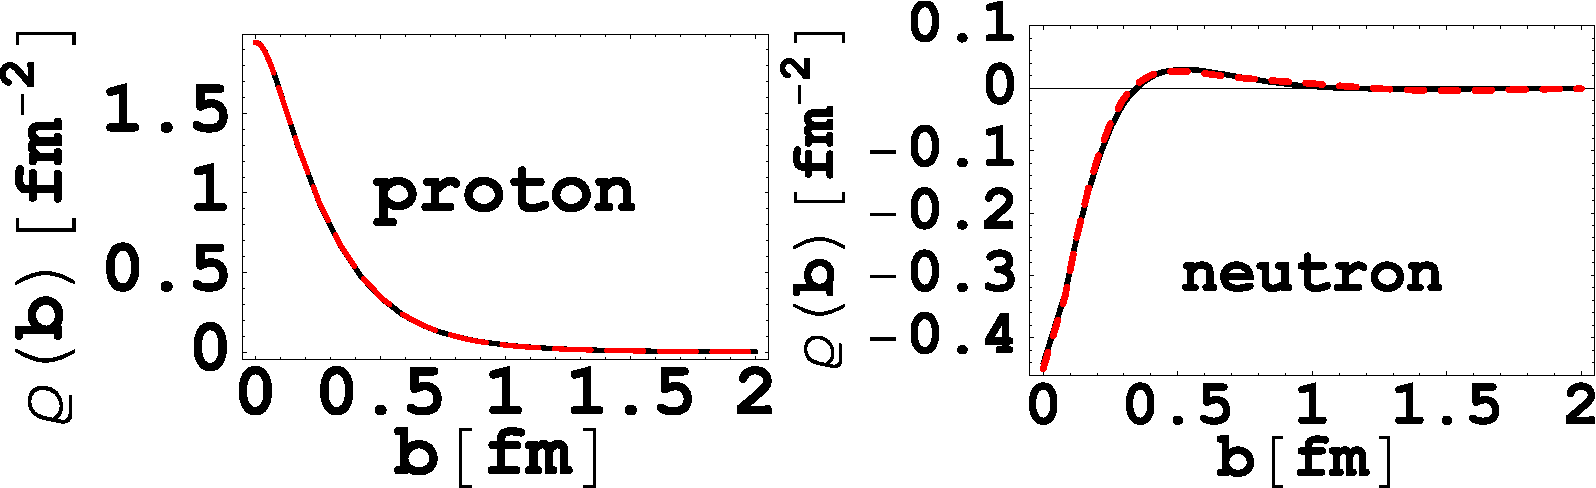
\includegraphics[width=0.9\linewidth]{charge_distribution_rotated}
	\caption{The proton charge density (left panel) and neutron charge density
		(right panel). Taken from Ref.~\cite{miller2007}}.
	\label{fig:charge}
\end{figure}
These results further demonstrate the internal structure of the nucleon.

In the 1960s, the quark model is proposed independently by Gell-Mann \cite{gell-mann1964} and Zweig  \cite{zweig1964a, zweig1964} to understand the growing number of new particles discovered through out
the 1940s and 1950s.
In the quark model, the baryons are made up of three quarks and the mesons are made up
of a quark and an antiquark, and can be organized as shown in \cref{fig:Octet}.
The magnetic moment of the proton can then be expressed as the sum of the magnetic moment
from the individual quarks. The proton consists of $uud$ and the neutron consists of $udd$,
requiring the wavefunction is symmetric in both flavor and spin, the wavefunction of a proton with
spin up is given by
\begin{equation}
	\begin{split}
		\ket{p:\frac{1}{2} \frac{1}{2}}=&  \Bigl\{\frac{1}{2}(\uparrow\downarrow\uparrow-\uparrow\uparrow\downarrow)(udu-uud) + \frac{1}{2}(\uparrow\uparrow\downarrow-\uparrow\downarrow\uparrow)(uud-udu)\\
		&+\frac{1}{2}(\uparrow\uparrow\downarrow-\downarrow\uparrow\uparrow)(uud-duu)\Bigl\} \frac{\sqrt{2}}{3}.
	\end{split}
\end{equation}
And the magnetic moments are now given by
\begin{align}
	\mu_p & = \frac{4}{3}\mu_u-\frac{1}{3}\mu_d,  \\
	\mu_n & = -\frac{1}{3}\mu_u+\frac{4}{3}\mu_d.
\end{align}
If we then also assumed the the $u$ and $d$ quarks share the same mass, the quark model
then predicts the ratio $\mu_p/\mu_n=-2/3$ which is impressively close to the measured ratio
\num{0.6849793(3)}\cite{workman2022}.
\begin{figure}[h!]
	\centering
	\begin{subfigure}{0.45\linewidth}
		\begin{picture}(150, 150)(-100, -100)
	\put(-25,42){\line(-3,-5){25}}
	\put(-25, 42){\line(1, 0){50}}
	\put(25, 42){\line(3,-5){25}}
	\put(-25, -42){\line(1,0){50}}
	\put(-25, -42){\line(-3, 5){25}}
	\put(25, -42){\line(3, 5){25}}

	\put(-25, 42){\circle*{3}}
	\put(-25, -42){\circle*{3}}
	\put(25, 42){\circle*{3}}
	\put(25, -42){\circle*{3}}
	\put(-50, 0){\circle*{3}}
	\put(50, 0){\circle*{3}}
	\put(0, 3){\circle*{3}}
	\put(0, -3){\circle*{3}}

	\put(-28, 47){$n$}
	\put(28, 47){$p$}
	\put(-28, -55){$\Xi^{-}$}
	\put(28, -55){$\Xi^{0}$}
	\put(55, 0){$\Sigma^{+}$}
	\put(-65, 0){$\Sigma^{-}$}
	\put(0, 10){$\Sigma^{0}$}
	\put(0, -15){$\Lambda$}

	\put(-120, 43){$s=0$}
	\put(-120, 0){$s=-1$}
	\put(-120, -43){$s=-2$}

	\put(-20, -85){$q=-1$}
	\put(45, -85){$q=0$}
	\put(70, -30){$q=1$}
\end{picture}

		\caption{The Baryon Octet}
	\end{subfigure}
	\begin{subfigure}{0.45\linewidth}
		\begin{picture}(150, 150)(-100, -100)
	\put(-25,42){\line(-3,-5){25}}
	\put(-25, 42){\line(1, 0){50}}
	\put(25, 42){\line(3,-5){25}}
	\put(-25, -42){\line(1,0){50}}
	\put(-25, -42){\line(-3, 5){25}}
	\put(25, -42){\line(3, 5){25}}

	\put(-25, 42){\circle*{3}}
	\put(-25, -42){\circle*{3}}
	\put(25, 42){\circle*{3}}
	\put(25, -42){\circle*{3}}
	\put(-50, 0){\circle*{3}}

	\put(50, 0){\circle*{3}}
	\put(0, 3){\circle*{3}}
	\put(0, -3){\circle*{3}}

	\put(-28, 47){$K^{0}$}
	\put(28, 47){$K^{+}$}
	\put(-28, -55){$K^{-}$}
	\put(28, -55){$\overline{K}^{0}$}
	\put(55, 0){$\pi^{+}$}
	\put(-65, 0){$\pi^{-}$}
	\put(0, 10){$\pi^{0}$}
	\put(0, -15){$\eta$}

	\put(-120, 43){$s=1$}
	\put(-120, 0){$s=0$}
	\put(-120, -43){$s=-1$}

%	\put(-20, -85){$q=-1$}
%	\put(45, -85){$q=0$}
%	\put(70, -30){$q=1$}
\end{picture}

		\caption{The Meson Octet}
	\end{subfigure}
	\caption{Baryons and meson organized based on their charge(diagonal), strangeness(vertical) and isospin $I_3$(horizontal). }
	\label{fig:Octet}
\end{figure}
These quarks would also carry a fractional charge ($2/3$ for $u$, $s$ quarks and $-1/3$ for $d$ quarks) to
explain the charge of the baryons. Since a fractional charged particles were never observed, and there were
no experimental evidence for a free quarks, the quark model was not considered as physical, but only a mathematical construct at the time.
\section{Deep Inelastic Scattering}
\label{sec:dis}
Evidence of the point-like constituents in the nucleon would later come from the deep
inelastic scattering (DIS) experiments \cite{breidenbach1969}, where a high
energy lepton ($l$) is inelastically scattered off a nucleon ($N$), as
illustrated in \cref{fig:DIS}
\begin{equation}
	l + N \rightarrow l^\prime + X.
\end{equation}
\begin{figure}[htbp!]
	\centering
	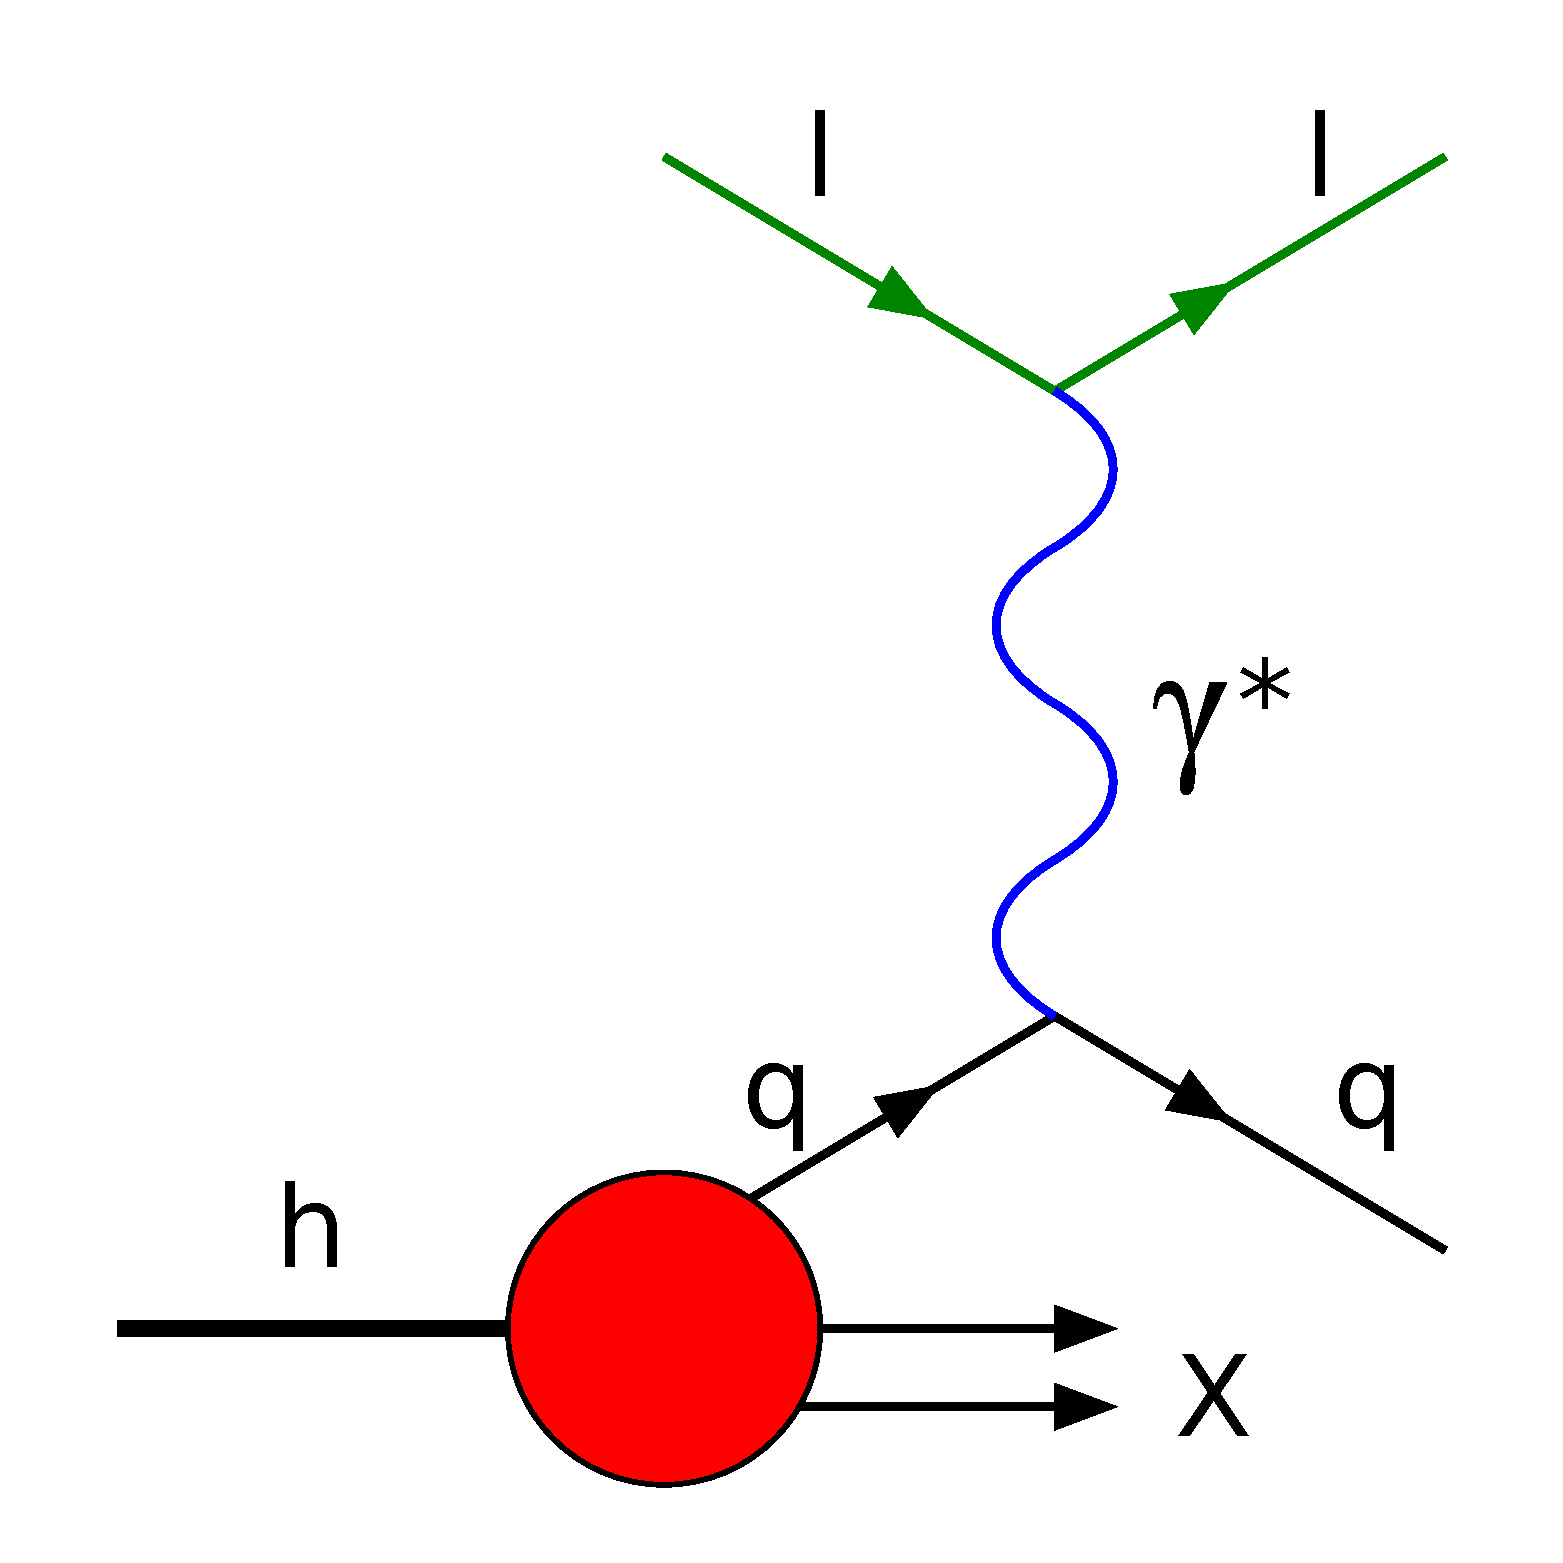
\includegraphics[width=0.3\linewidth]{DIS}
	\caption{The Feynman diagram for DIS}
	\label{fig:DIS}
\end{figure}
Similar to \cref{eq:ep_cs}, the DIS cross section can be expressed as
\begin{equation}
	\eval{\frac{d^2\sigma}{dE^\prime d\Omega}}_{DIS} = \frac{\alpha^2}{4E^2 \sin^4
		\frac{\theta}{2}} \left[ W_2\left(\nu,Q^2\right)\cos^2
		\frac{\theta}{2} + W_1\left(\nu,Q^2\right)\sin^2 \frac{\theta}{2}
		\right],
	\label{eq:DIS_cs1}
\end{equation}
where $\nu$ is the energy transferred by the scattering lepton.
In the elastic scattering, the cross section only depends on the momentum transfer squared $Q^2$,
as the energy transfer in $\nu$ is related to momentum transfer by $Q^2=2M\nu$.
In DIS, this relation no longer holds and the cross section would also depends on $\nu$.

It is also customary to define the structure functions $F_{1,2}$ from $W_{1,2}$ as:
\begin{equation}
	\begin{split}
		F_1\left(x,Q^2\right) &= MW_1\left(\nu,Q^2\right),\\
		F_2\left(x,Q^2\right) &= \nu W_2\left(\nu,Q^2\right),
	\end{split}
\end{equation}
where $x=Q^2/2M\nu$ and $M$ is the mass of the nucleon. It was observed that at sufficiently high $Q^2$,
these structure functions $F_{1,2}$ are independent of $Q^2$, as illustrated in
\cref{fig:w2}. \Cref{fig:w2} shows the early measurements of the
structure function $F_2=\nu W_2$ as a function of $Q^2$ for a fixed
$x=1/\omega=0.25$ taken from Ref.~\cite{friedman1972}. This observation is
known as Bjorken scaling \cite{bjorken1969}.
\begin{figure}[htpb!]
	\centering
	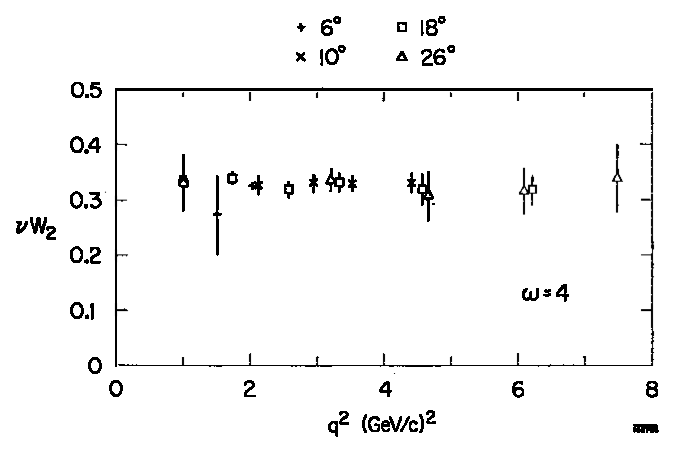
\includegraphics[width=0.5\linewidth]{nu_W2}
	\caption{Early measurement structure function $F_2=\nu W_2$ from
		fixed-target electron-proton inelastic scattering at SLAC for
		$x=1/\omega=0.25$ taken from Ref.~\cite{friedman1972}. The observation
		that $F_2(x,Q^2)$ is independent of $Q^2$ is known as Bjorken scaling. }
	\label{fig:w2}
\end{figure}
Taking the interpretation that the structure function are related to the form factors in elastic scattering,
and therefore the Fourier transform of the charge distribution, the Bjorken scaling would suggest
the existence of point-like particles in the proton

\section{Parton Model}
\label{sec:parton}
To explain the scaling behavior, Feynman proposed the parton model \cite{feynman1969}.
In this model, hadrons are treated as extended objects which are made up of point-like
constituents (partons) held together by their mutual interaction. We now know
these partons are quarks and gluons described by QCD, but this was not known at
the time. Consider the DIS process, the hadron is Lorentz contracted in the
direction of the collision in the center-of-mass frame, and the internal
interaction are time dilated. As the center-of-mass energy increases, the
lifetime of the virtual partonic state is lengthened, and the time for the
electron to pass trough the hadron is shortened. If the lifetime of the virtual
partonic states is longer than the duration of the electron-hadron interaction,
the partons are essentially frozen and the parton-parton interactions are
neglectable. The hadrons can be considered as a collection of ``free'' partons,
and each parton may be thought of as carrying a definite fraction $x$ of the
hadron's momentum. The high energy lepton in DIS can be treated as scattering
off these partons elastically. The electron-parton elastic scattering can be
calculated using perturbative QCD, whereas the non-perturbative long-range
interaction within the hadron is encapsulated in the Parton Distribution
Function (PDF) $f_{a/h}\left(x\right)$, which can be interpreted as the probability
of finding a parton of species $a$ in hadron $h$ with fraction $x$ of the hadron's momentum.
And the cross section can be written as a convolution
of the non-perturbative PDF and the perturbative short range interaction. To leading
order, the structure function $F_2\left(x,Q^2\right)$ is given by
\begin{equation}
	F_2\left(x,Q^2\right)=x\sum_i e^2_i f_i\left(x,Q^2\right),
	\label{eq:F2_parton}
\end{equation}
where $e_i$ is the charge carried quark and antiquark of flavors $i$. Since the
gluon does not carry any charge, it does not enter the cross section at leading
order. The ability to write the structure function and the cross section as a
convolution of the non-perturbative PDF and pertubative short range interaction
is known as the factorization theorem \cite{collins1989}. These PDFs are also
expected to be universal and independent of the details of the scattering
process, as they describe the dynamics of the partons in a given hadron.

In the parton model, the structure functions $F_2$ and $F_1$ are clearly related. And
from \cref{eq:DIS_cs1}, the structure function $F_1$ is
related to the magnetic form factor $G_M$ in \cref{eq:ep_cs}. If the partons
are spin 0 particles, one would expect $F_1$ to be zero. In leading order of QCD,
only the quarks and antiquarks contribute to the cross section. Since quarks and
antiquarks are spin 1/2 particles, this relation is given by the Callan-Gross
relation \cite{callan1968,callan1969}
\begin{equation}
	F_2\left(x\right) = 2x F_1\left(x\right).
	\label{eq:CS_relation}
\end{equation}
The measured deviation of the Callan-Gross relation, defined as
\begin{equation}
	K_0 = \frac{F_2}{2xF_1}-1,
\end{equation}
is shown in \cref{fig:callan_gross}, taken from Ref.~\cite{kendall1991}.
For large $Q^2$, $K_0$ is consistent with zero, establishing the spin of the
charged partons is 1/2.
\begin{figure}[htbp!]
	\centering
	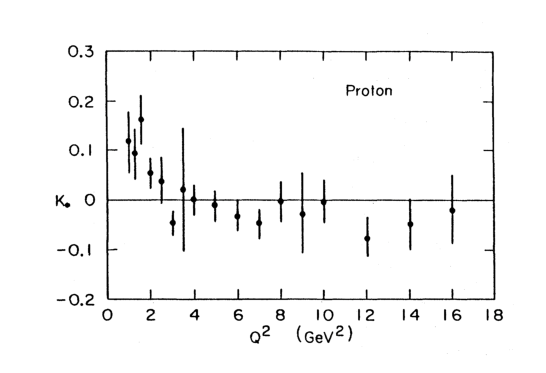
\includegraphics[width=0.5\linewidth]{Callan_Gross_relation}
	\caption{The deviation from the Callan-Gross relation, defined as
		$K_0=F_2/2xF_1 -1$, taken from Ref.~\cite{kendall1991}. This result
		demonstrates the spin 1/2 nature of the partons.}
	\label{fig:callan_gross}
\end{figure}
The deviation at low $Q^2$ is expected from the QCD corrections and contributions from
the gluons.

\section{Sum Rules}
\label{sec:sum_rules}
Since hadrons are characterized by their quantum numbers, and these quantum numbers
are carried by the constituent partons, these quantum numbers serve as constraints
on these PDFs. For example, using the numbers of valence quarks in the protons,
one can impose the following constraints
\begin{equation}
	\begin{split}
		\int_{0}^{1} \dd{x} \left[f_{u/p} \left(x\right)-f_{\bar{u}/p} \left(x\right)\right]&=2,\\
		\int_{0}^{1} \dd{x} \left[f_{d/p} \left(x\right)-f_{\bar{d}/p} \left(x\right)\right]&=1,\\
		\int_{0}^{1} \dd{x} \left[f_{i/p} \left(x\right)-f_{\bar{i}/p} \left(x\right)\right]&=0 \qquad \text{for other quark flavors } i.
	\end{split}
\end{equation}
And the momentum of the hadron should be distributed among the partons, hence
\begin{equation}
	\sum_{i=q,\bar{q},g}\int_{0}^{1} \dd{x} xf_{i/h}\left(x\right)=1.
\end{equation}
An important sum rule is the Gottfried sum rule \cite{gottfried1967}. It can be obtained
if we use the isospin symmetry to relate the neutron distributions to those of
the proton, namely the (anti) up quark in the neutron would have the same distribution
as (anti) down quark in proton, and vice-versa; the other quarks flavors and gluon
distribution would be the same in both proton and neutron.
\begin{equation}
	\begin{split}
		\bar{u}(x) &\equiv f_{\bar{u}/p}(x) = f_{\bar{d}/n}(x),\text{ and }\\
		\bar{d}(x) &\equiv f_{\bar{d}/p}(x) = f_{\bar{u}/n}(x).
	\end{split}
\end{equation}
Using this relation
\begin{equation}
	\begin{split}
		S_G & = \int_0^1 \frac{\dd{x}}{x}\left(F_2^{p}(x) - F_{2}^{n}(x)\right)\\
		& = \frac{1}{3} \int_0^1 \dd{x} \left[u\left(x\right) - d\left(x\right)
			+ \bar{u}\left(x\right) - \bar{d}\left(x\right)\right]\\
		& = \frac{1}{3} \int_0^1 \dd{x} \left[u\left(x\right) - \bar{u}\left(x\right)\right]
		- \frac{1}{3} \int_0^1 \dd{x} \left[d\left(x\right) - \bar{d}\left(x\right)\right]
		+ \frac{2}{3} \int_0^1 \dd{x} \left[\bar{u}\left(x\right)-\bar{d}\left(x\right)\right]\\
		& = \frac{1}{3} + \frac{2}{3} \int_0^1 \dd{x} \left[\bar{u}\left(x\right)-\bar{d}\left(x\right)\right].
	\end{split}
\end{equation}
If one made the naive assumption that $\bar{u}\left(x\right)= \bar{d}\left(x\right)$,
then $S_G$ would be expected to be $1/3$. And this assumption can be tested using DIS.
One of the early measurements is from the New Muon Collaboration (NMC) \cite{amaudruz1991}.
The measured $F_2^p-F_2^n$ by NMC is shown in \cref{fig:NMC_Gottfried}.
\begin{figure}[htbp!]
	\centering
	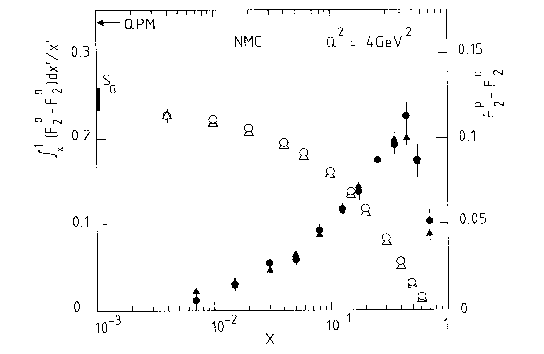
\includegraphics[width=0.7\linewidth]{Gottfried}
	\caption{The difference $F_2^p -F_2^n$ (solid and scale to the right) and
		$\int_{x_{min}}^1 (F_2^p-F_2^n)\dd{x}/x$ (open and scale to the left)
		determined by NMC, taken from Ref.~\cite{amaudruz1991}. The extrpolation
		to $x_{min}=0$ is indicated by the bar.}
	\label{fig:NMC_Gottfried}
\end{figure}
The measured Gottfried sum is $0.240 \pm 0.016$, which is significantly below
$1/3$, suggesting an asymmetry in the light sea-quarks, $\bar{d}(x)\neq \bar{u}(x)$.

\section{Quantum Chromodynamics}
\label{sec:QCD}
\pdfmargincomment{General QCD}
Quantum Chromodynamics (QCD) is a theory of the strong interactions. It was
introduced by Fritzsch and Gell-Mann \cite{fritzsch1972} and Fritzsch, Gell-Mann,
and Leutwyler \cite{fritzsch1973}. QCD is a non-abelian gauge theory with an
$SU(3)$ gauge symmetry applied to the color degree of freedom. The $SU(3)$ group
chosen to account for (a) meson states made up of $q\bar{q}$ but not $qq$ bound states.
(b) There must color singlet states. (c) The number of colors for each flavor
must be in agreement with the measured hadronic $e^+ e^-$ cross-section.


An important feature of QCD is the asymptotic freedom. Being a renormalizable
theory, a regularization procedure and a set of renormalization prescription
need to be specified. In the renormalization process, the renomalized coupling $\alpha$
is introduced and this coupling would be a function of the renomalization scale $\mu$.
It is noted that the coupling constant vanishes as $Q/\mu$ tends to infinity,
allowing perturbative expansion of QCD at large $Q$.


\subsection{QCD Improved Parton Model and Scaling Violation}
\label{subsec:scaling_violation}
In QCD, the parton distribution functions can be defined as matrix elements of
operators acting on the hadron state. These operators act to count the number of
quarks and gluon carrying a fraction $\xi$ of the hadron's momentum. For quarks,
the distribution is given by \cite{collins1989}
\begin{equation}
	f_{q/h}\left(\xi\right) = \frac{1}{4\pi}\int \dd{x} e^{-i\xi P^{+} x^{-}} \mel{P}{\bar{\psi}\left(0,x^-,0_\perp\right)\gamma^+ \mathcal{G} \psi\left(0,0,0_\perp\right)}{P},
\end{equation}
where $\mathcal{G}$ is the gauge link operator
\begin{equation}
	\mathcal{G}=\mathcal{P} \exp \left\{ ig\int_0^{x^-}\dd{y^-} A_c^+ \left(0,y^-,0_\perp\right)t_c\right\},
\end{equation}
where $\mathcal{P}$ denoted the path ordering of the gluon field operators $A_a^+$
along the path. Similarly, the gluon distribution function is given by
\begin{equation}
	f_{g/h}\left(\xi\right) = \frac{1}{2\pi\xi P^+}\int \dd{x} e^{-i\xi P^{+} x^{-}} \mel{P}{\tensor{F_a\left(0,x^-,0_\perp\right)}{^+^\nu}\gamma^{+} \tensor{\mathcal{G}}{_a_b} \tensor{F_b\left(0,0,0_\perp\right)}{_\nu^+}}{P},
\end{equation}
where $F^a_{\mu\nu}$ is the field operator, and the octet representation of the $SU(3)$
generating matrices $t_c$ is used in $\mathcal{G}$.

The QCD generalization of \cref{eq:F2_parton} is given
\begin{equation}
	\frac{1}{x}F_2\left(x,Q^2\right) = \sum_a \int_x^1 \frac{\dd{\xi}}{x}f_{a/h}\left(\xi,\mu\right)\frac{\xi}{x}H_{2a}\left( \frac{x}{\xi}, \frac{Q}{\mu}, \alpha_s\left(\mu\right)\right)
	+ \text{Remainder}
\end{equation}
The hard scattering coefficient $H_{2a}$ would be power series in $\alpha_s$. It
can be shown the remainder is suppress by powers of $Q$. Here the parton
distribution also depends on the renormalization scale $\mu$. This scale
dependency is introduce by the renomalization procedure. By requiring the cross
section and the structure functions to be independent of the scale $\mu$,
one can show that the renormalization group equation for the distribution
functions is
\begin{equation}
	\mu\frac{d}{d\mu}f_{a/h}\left(\xi,\mu\right)=\sum_b \int_\xi^1 \frac{\dd{\zeta}}{\zeta} P_{a/b}\left(\zeta,\alpha_s\left(\mu\right)\right) f_{b/h}\left(\frac{\xi}{\zeta},\mu\right),
\end{equation}
where $P_{a/b}$ is the Altarelli-Parisi kernel \cite{altarelli1977}.

At order $\alpha_s$, the $F_2$ structure function is given by \cite{collins1989}
\begin{equation}
	\frac{1}{x} F_2\left(x,Q^2\right) = \sum_j e^2_j f_{j/h}\left(x,\mu\right) + \sum_{j,b} e^2_j \int^1_x \frac{\dd{\xi}}{\xi} f_{b/h}\left(x,\mu\right) \frac{\alpha_s}{\pi} C_{jb}\left(\frac{x}{\xi}, \frac{Q}{\mu}\right) + \mathcal{O}(\alpha_s^2).
\end{equation}
The sums over $j$ runs over the quarks and antiquarks flavors. While the gluons
did not contribute at leading order, they contribute at order $\alpha_s$ through
virtual quark-antiquark pairs. The hard scattering coefficients $C_{jb}$ are
given by
\begin{align}
	C_{jk}(z,1) & = \delta_{jk} \frac{4}{3} \left[ -\frac{1}{2}\frac{1+z^2}{1-z} \ln\left(\frac{z}{1-z}\right) + \frac{3}{4} \frac{1}{1-z} -\frac{3}{2} -z\right]_+ \\
	C_{jg}(z,1) & = -\frac{1}{2} \left\{ \frac{1}{2}\left[z^2+(1-z)^2\right] \left[\ln\left(\frac{z}{1-z}\right)+1\right] -3z(1-z)\right\},
\end{align}
where the plus sign denote the subtraction that regulate the $z\rightarrow1$
singularity,
\begin{equation}
	\begin{split}
		\int^1_x \dd{z} \left[C(z)\right]_+ h(z) &= \int_0^1 \dd{z} \left[C(z)\right]_+ h(z)\Theta(z>x)\\
		& = \int_0^1 \dd{z} C(z) \left\{h(z)\Theta(z>x) -h(1)\right\}.
	\end{split}
\end{equation}

It is customary to choose $\mu =Q$ to avoid large logarithms of $\mu /Q$ in the
power expansions of $H$. As such the $\mu$ dependency in the parton distribution
functions can be interpreted as a virtual photon with higher $Q$ would probe the
nucleon with better resolution.

\Cref{fig:DIS_scaling} shows the extracted $F_2$ from DIS measurements and compared
with the NLO calculation. The $Q^2$ dependency is known as scaling violation and
originates from higher order corrections and $Q$ dependency of the PDF.
\begin{figure}[h!]
	\centering
	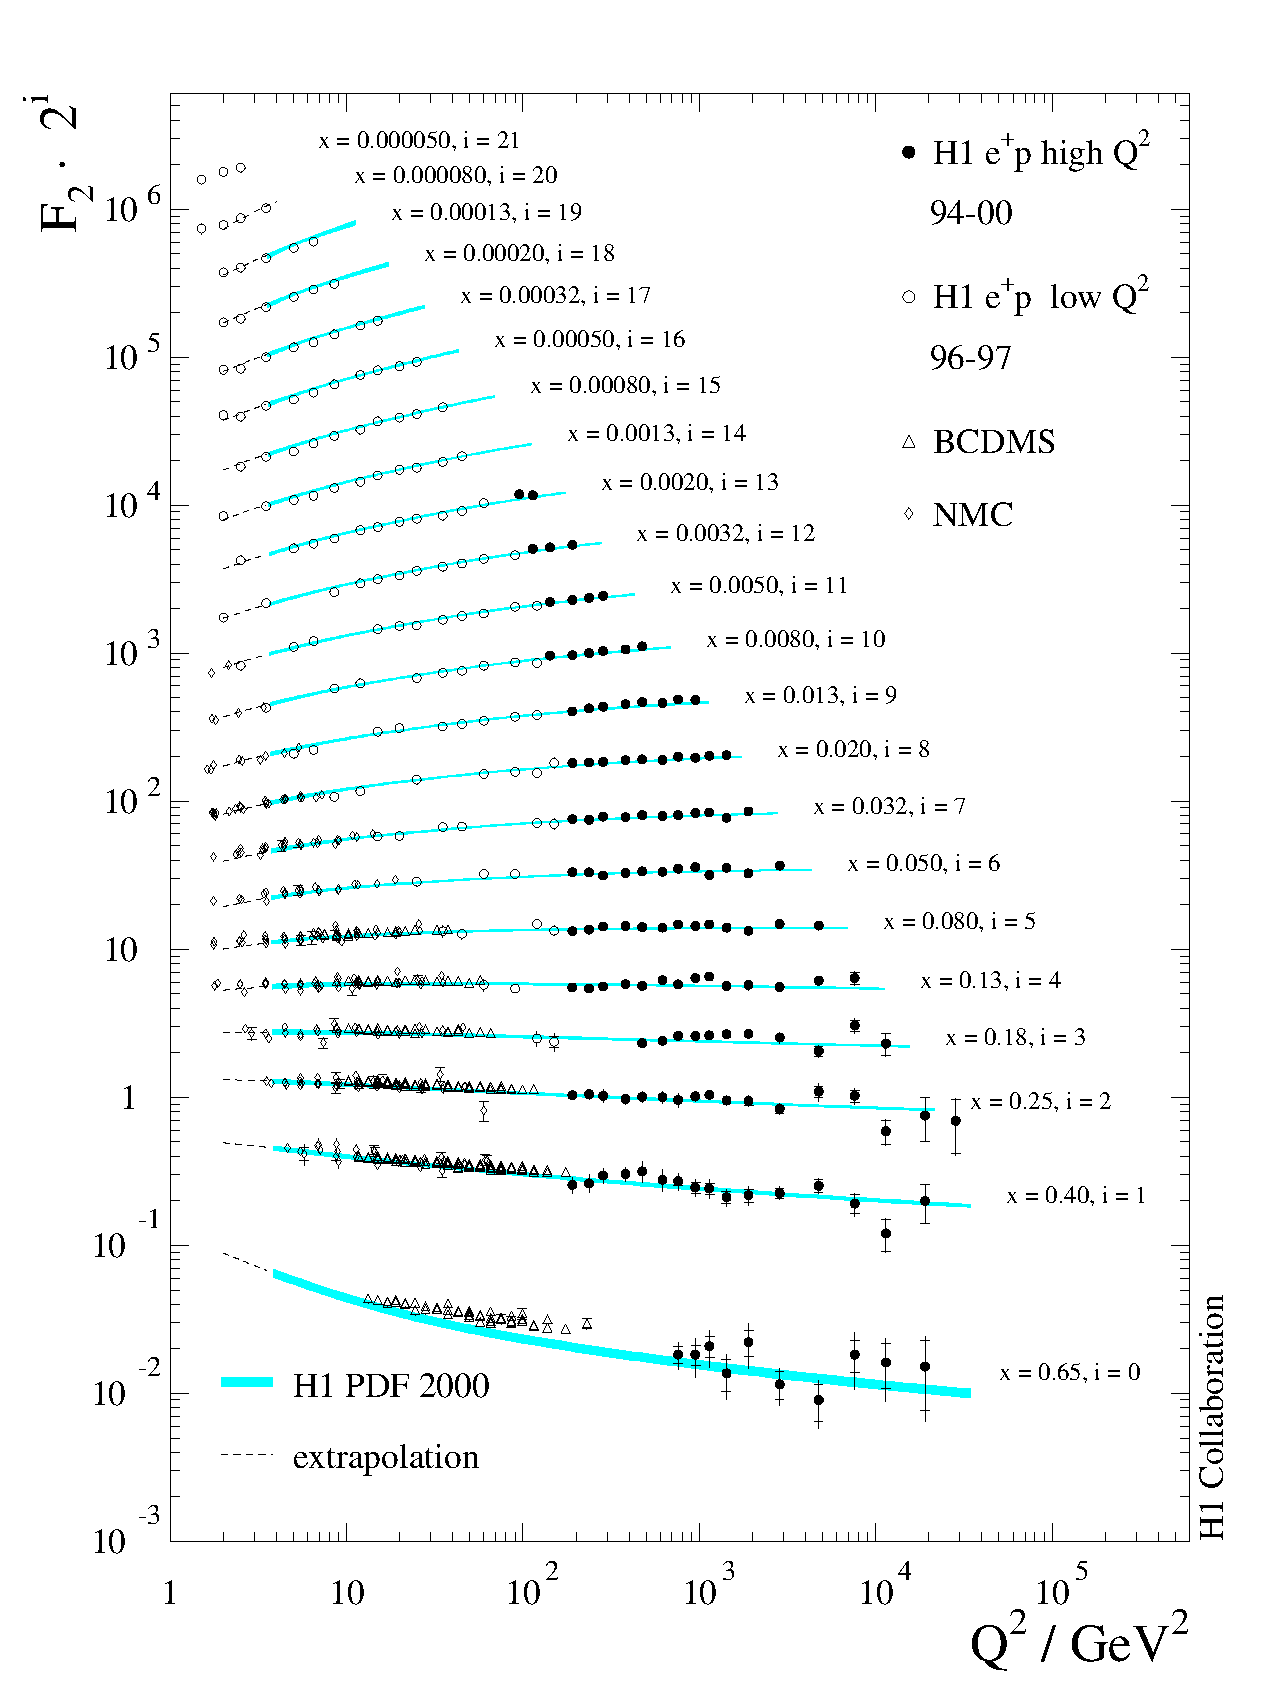
\includegraphics[width=0.5\linewidth]{DIS_scaling}
	\caption{
		Compilation of data on DIS, and compared with NLO calculations.
		Taken from Ref.~\cite{adloff2003}
		The $Q^2$ dependency is known as scaling violation,
		and originates from higher order corrections and $Q$ dependency of the PDF.
	}
	\label{fig:DIS_scaling}
\end{figure}
The Gottfried Sum Rule introduced in \cref{sec:sum_rules} would also be modified due to
QCD effects. At order $\alpha_s^2$, in the limit of a symmetric sea, the Gottfried Sum Rule
is given by \cite{kataev2003}
\begin{equation}
	I_{GSR} = \begin{cases}
		\frac{1}{3}\left[ 1 + 0.0355\left(\frac{\alpha_s}{\pi}\right)-0.811\left(\frac{\alpha_s}{\pi}\right)^2 \right] & n_f=3, \\
		\frac{1}{3}\left[ 1 + 0.0384\left(\frac{\alpha_s}{\pi}\right)-0.822\left(\frac{\alpha_s}{\pi}\right)^2 \right] & n_f=4,
	\end{cases}
\end{equation}
where $n_f$ is the active flavor.
Taking $\alpha_s(Q^2)\approx 0.35$, the numerical value is $\approx 0.3313$. Therefore,
the light sea-quark asymmetry is still needed to explained the NMC result.

\Cref{fig:CT18_scale} shows the PDF extracted by CTEQ-TEA collaboration in their
CT18 global analysis \cite{hou2021}. The sea-quarks from the gluon splitting
can be seen at low $x$ and is more important at large $Q$. This demonstrate the
QCD evolution of the PDF.

\begin{figure}
	\centering
	\begin{subfigure}{0.45\linewidth}
		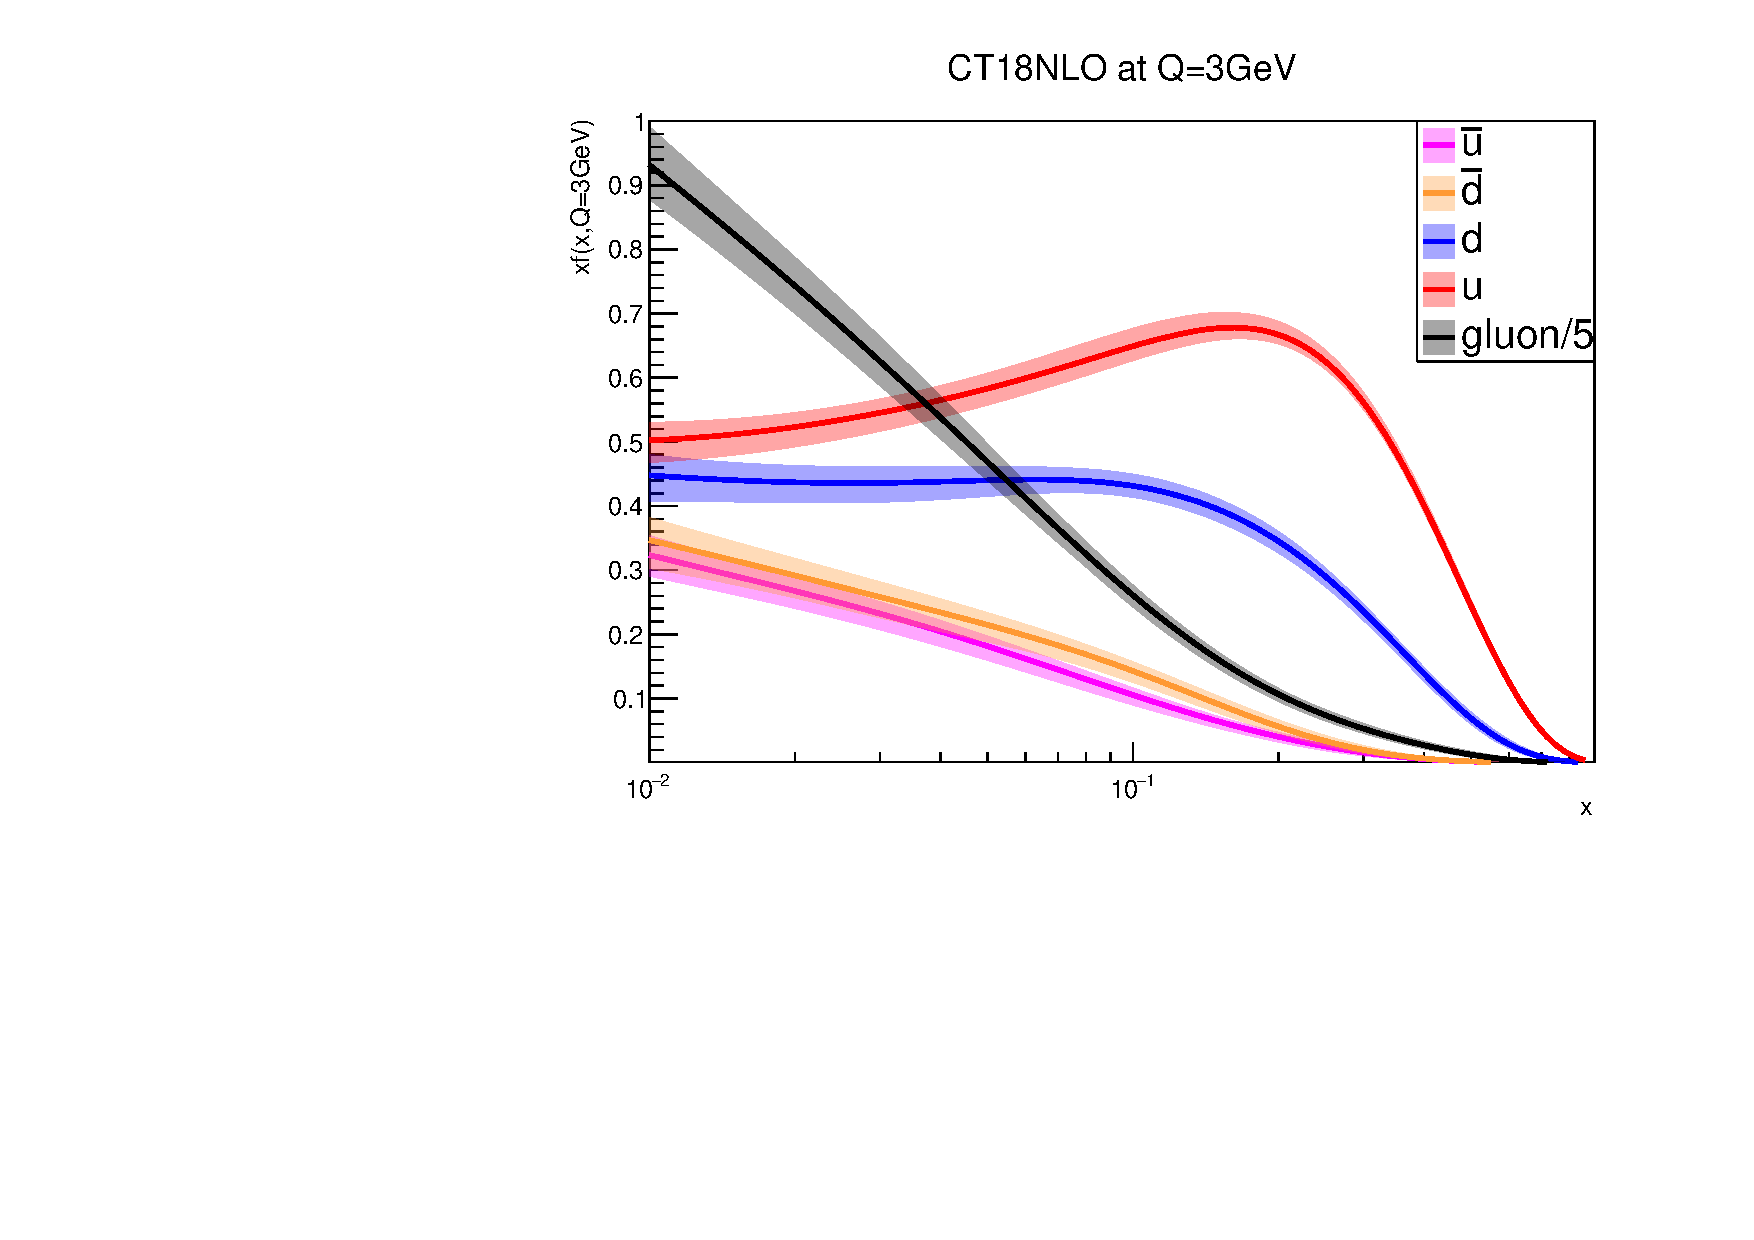
\includegraphics[width=\linewidth]{CT18NLO}
	\end{subfigure}
	\begin{subfigure}{0.45\linewidth}
		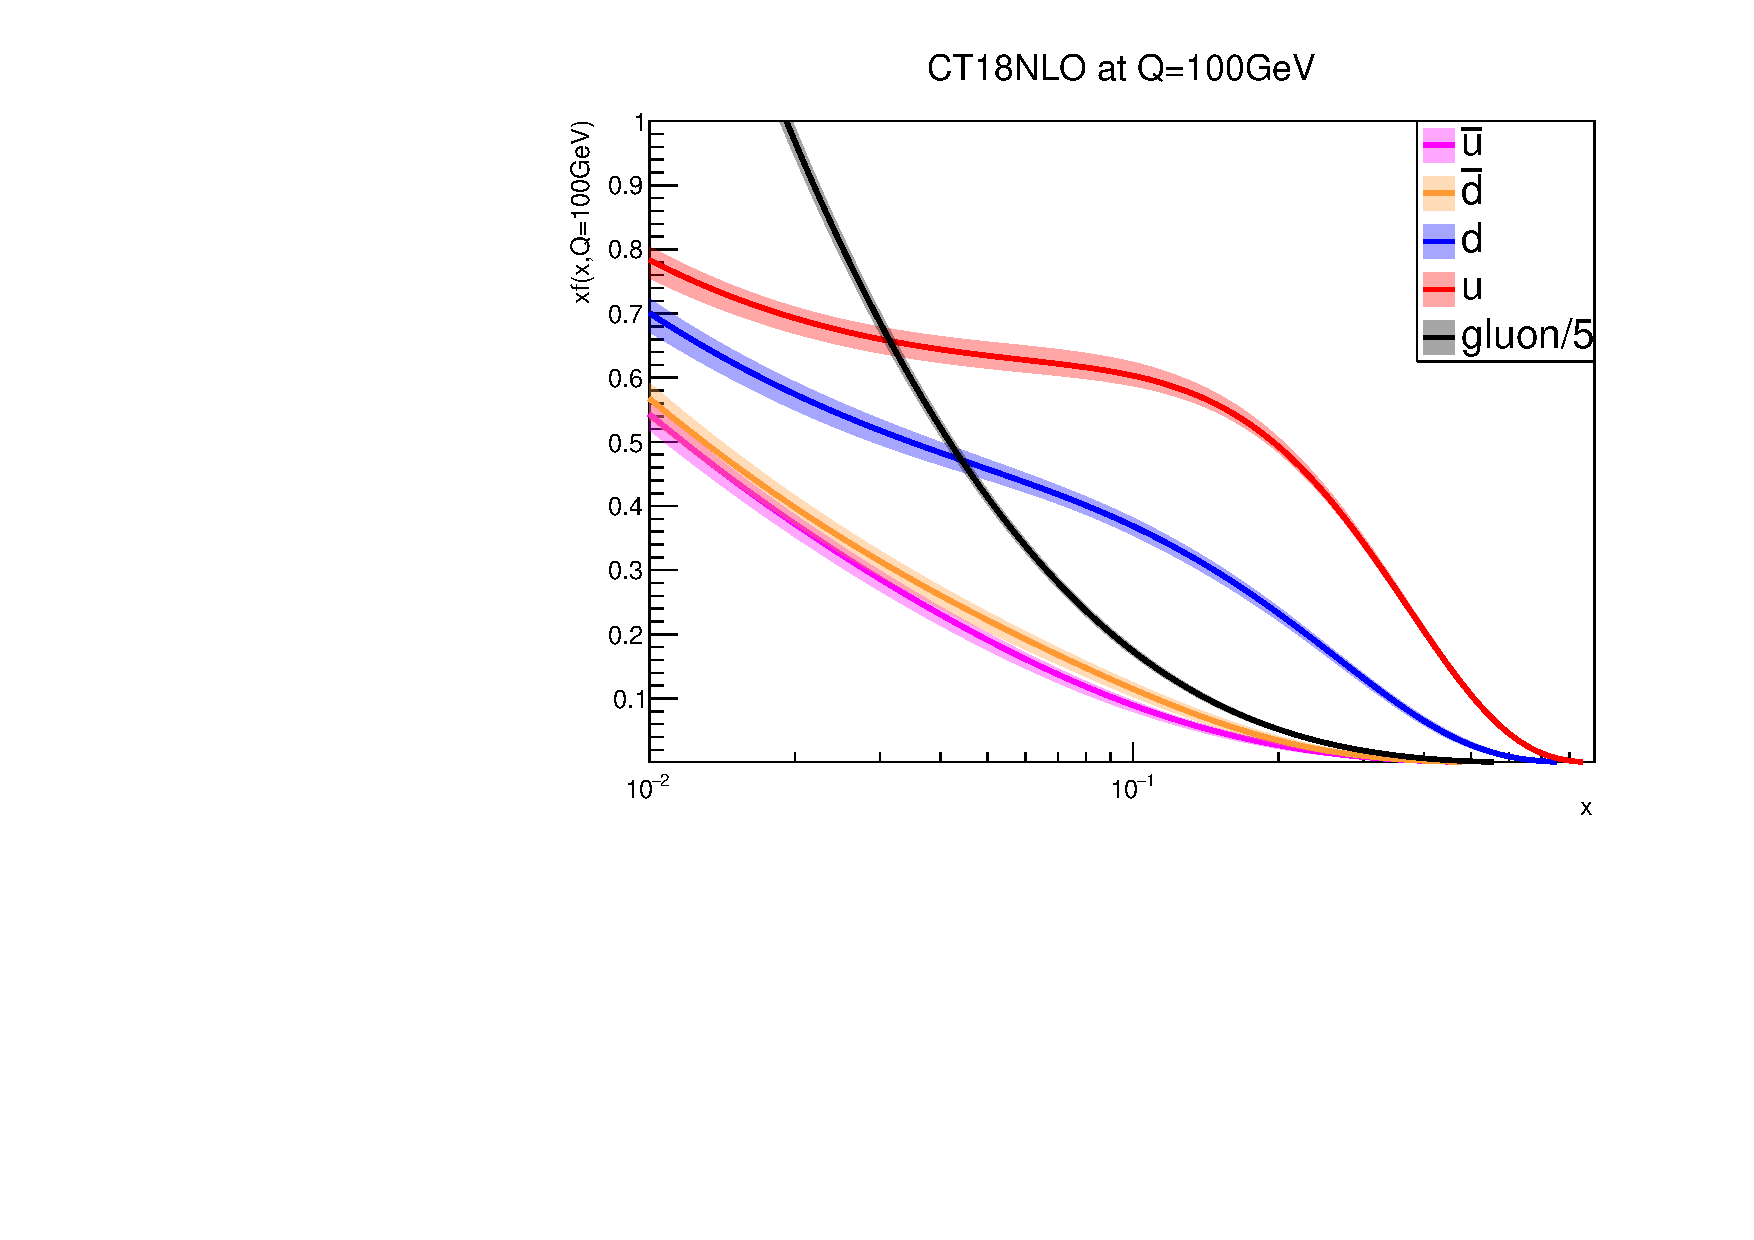
\includegraphics[width=\linewidth]{CT18NLO_100}
	\end{subfigure}
	\caption{The parton distribution function from CT18 \cite{hou2021} global analysis at two different scale.
		The gluon distribution is scale down by a factor of 5.}
	\label{fig:CT18_scale}
\end{figure}


\chapter{Drell-Yan Process}
\label{ch:DY}
Another process for probing the hadron structure is the Drell-Yan process \cite{drell1970}.
As illustrated in \cref{fig:DY}, this process involves two partons from the
two colliding hadrons to annihilate and form a lepton pair.
\begin{equation}
	h_A + h_B \rightarrow l + \bar{l} + X.
\end{equation}
The Drell-Yan process is related to the DIS process via crossing symmetry.
\begin{figure}[htbp!]
	\centering
	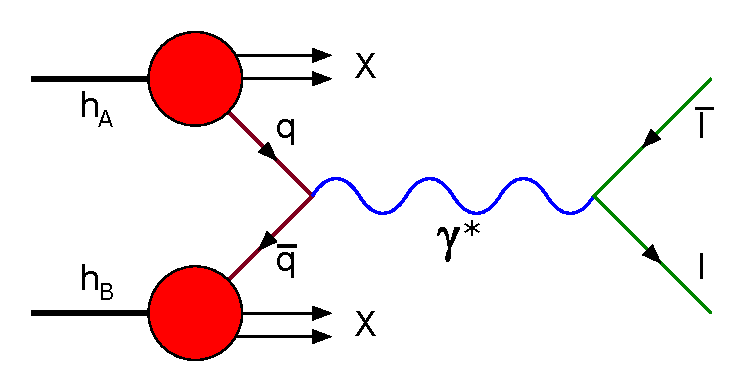
\includegraphics[width=0.5\linewidth]{Drell-Yan}
	\caption{The leading order Feynman diagram for the Drell-Yan process}
	\label{fig:DY}
\end{figure}
Similar to DIS, the Drell-Yan cross section can be factorized into the non-perturbative
PDF and the perturbative parton-parton scattering. And the proof of factorization
theorem for Drell-Yan can be found in Ref.~\cite{collins1989}. At leading-order,
the cross section can be written as
\begin{equation}
	\frac{d^2\sigma_{DY}}{dx_{1}dx_{2}} = \frac{4\pi\alpha^2}{9M^2}\sum_i e^2_i
	\left[f_{i/A}\left(x_1\right)f_{\bar{i}/B}\left(x_2\right) +
	f_{\bar{i}/A}\left(x_1\right)f_{i/B}\left(x_2\right)
	\right],
	\label{eq:DY_cs}
\end{equation}
where $M$ is the mass of the lepton pair, $x_1$ and $x_2$ are the momentum fraction
carried by the partons from the two colliding hadrons. To simplify the notation,
the scale dependence $Q^2$ of the PDF is omitted here. In fixed target environments,
the scale $Q^2$ is typically chosen to the dilepton mass squared.
The mass of the lepton pair and momentum fractions can be related through the following
\begin{equation}
	M^2= sx_1x_2,
	\label{eq:mass}
\end{equation}
where $s$ is the hadron-hadron center mass energy squared.
Since the underlying mechanism for the Drell-Yan process at leading order involves the annihilation
of a quark and antiquark, this process is particularly useful in probing the antiquark
content of the hadron.
In the parton model, the angular distribution of the Drell-Yan dilepton would have the following
distribution from the decay of the transversely polarized virtual photon,
\begin{equation}
	\dv{\sigma_{DY}}{\Omega} = \sigma_0(1+\lambda \cos^2\theta),
\end{equation}
where $\theta$ is the polar angle of the lepton in the virtual photon rest frame and $\lambda=1$.

The Drell-Yan process and the parton model has been successful in explaining the shape of
the dimuon production cross section and the angular distribution in early experiments. However,
the  experimental cross section was about a factor of two larger than predicted, and the
transverse momentum of the dilepton is larger than expected from the convolution of the intrinsic
parton momenta \cite{mcgaughey1999}. These discrepancies can be resolved if higher order
QCD correction is included.
\begin{figure}[htbp!]
	\centering
	\begin{subfigure}{0.45\linewidth}
		\centering
		\begin{tikzpicture}
	\tikzstyle{every node}=[font=\large]
	\begin{feynman}
		\vertex  (a1){$q$};
		\vertex [right= 4cm of a1] (a2) {$\gamma^*$};
		\vertex [below= 4cm of a1] (b1) {$\bar{q}$};
		\vertex[below= 4cm of a2] (b2) {$g$};
		\vertex  at ($(a1) + (2cm , -1cm)$) [dot] (d);
		\vertex [below= 2 cm of d] (d1);
		\diagram*{
		(a1) --[fermion](d),
		(d1) --[fermion](b1),
		(d) --[fermion] (d1),
		(d1) --[gluon](b2),
		(d) --[photon](a2);
		};
	\end{feynman}
\end{tikzpicture}

		\caption{Gluon bremstrahlung}
	\end{subfigure}
	\begin{subfigure}{0.45\linewidth}
		\centering
		\begin{tikzpicture}
	\tikzstyle{every node}=[font=\large]
	\begin{feynman}
		\vertex  (a1){$q$};
		\vertex at ($(a1) + (1cm, -1cm)$) (a2);
		\vertex [below= 4cm of a1] (b1) {$\bar{q}$};
		\vertex [below= 2 cm of a2] (b2);
		\vertex at ($(a2) + (1cm, -1cm)$) (d);
		\vertex [right= 2 cm of d] (d1){$\gamma^*$};
		\diagram*{
		(a1) --[fermion](a2),
		(b2) --[fermion](b1),
		(a2) --[gluon] (b2),
		(a2) --(d),
		(b2) --(d),
		(d) --[photon](d1);
		};
	\end{feynman}
\end{tikzpicture}

		\caption{Interference from $\mathcal{O}(\alpha^2_s)$}
	\end{subfigure}

	\begin{subfigure}{\linewidth}
		\centering
		\begin{subfigure}{0.45\linewidth}
			\centering
			\begin{tikzpicture}
	\tikzstyle{every node}=[font=\large]
	\begin{feynman}
		\vertex  (a1){$q$};
		\vertex [right= 4cm of a1] (a2) {$q$};
		\vertex [below= 4cm of a1] (b1) {$g$};
		\vertex[below= 4cm of a2] (b2) {$\gamma^*$};
		\vertex  at ($(b1) + (1cm , +2cm)$) [dot] (d);
		\vertex [right= 2 cm of d] (d1);
		\diagram*{
		(a1) --[fermion](d),
		(b1) --[gluon](d),
		(d) --[fermion] (d1),
		(d1) --[fermion](a2),
		(d1) --[photon](b2);
		};
	\end{feynman}
\end{tikzpicture}

		\end{subfigure}
		\begin{subfigure}{0.45\linewidth}
			\centering
			\begin{tikzpicture}
	\tikzstyle{every node}=[font=\large]
	\begin{feynman}
		\vertex  (a1){$q$};
		\vertex [right= 4cm of a1] (a2) {$\gamma^*$};
		\vertex [below= 4cm of a1] (b1) {$g$};
		\vertex[below= 4cm of a2] (b2) {$q$};
		\vertex  at ($(a1) + (2cm , -1cm)$) [dot] (d);
		\vertex [below= 2 cm of d] (d1);
		\diagram*{
		(a1) --[fermion](d),
		(b1) --[gluon](d1),
		(d) --[fermion] (d1),
		(d1) --[fermion](b2),
		(d) --[photon](a2);
		};
	\end{feynman}
\end{tikzpicture}

		\end{subfigure}
		\caption{Gluon Compton scattering}
	\end{subfigure}
	\caption{Examples of diagrams contributing to the Drell-Yan cross section
		at NLO.}
	\label{fig:NLO_DY}
\end{figure}
At NLO ($\mathcal{O}\left(\alpha_s\right)$), diagram such as gluon bremsstrahlung
and Compton scattering begin to contribute, as shown in \cref{fig:NLO_DY}.
And the NLO expression can be written as a sum of the contribution from $q\bar{q}$
annihilation process
\begin{equation}
	\frac{d^2\sigma_A}{dQ^2dx_{F}} = \frac{4\pi\alpha^2}{9M^2} \sum_i e^2_i \int^1_{x_1} \dd{t_1} \int^1_{x_2} \dd{t_2}
	\left[ \frac{\hat{\sigma_{DY}}}{dQ^2dx_F}+\frac{\hat{\sigma_{A}}}{dQ^2dx_F} \right]
	\left[f_{i/A}\left(t_1\right)f_{\bar{i}/B}\left(t_2\right) +
	f_{\bar{i}/A}\left(t_1\right)f_{i/B}\left(t_2\right)
	\right],
\end{equation}
and Compton scattering process
\begin{multline}
	\frac{d^2\sigma_C}{dQ^2dx_{F}} = \frac{4\pi\alpha^2}{9M^2} \sum_i e^2_i \int^1_{x_1} \dd{t_1} \int^1_{x_2} \dd{t_2}
	\frac{\hat{\sigma_{C}}}{dQ^2dx_F}\left[ f_{g/A}\left(t_1\right)
	\left[f_{i/B}\left(t_2\right) +f_{\bar{i}/B}\left(t_2\right) \right]\right.
	\\\left.+\left[f_{i/A}\left(t_1\right) +f_{\bar{i}/A}\left(t_1\right) \right] f_{g/B}\left(t_2\right)\right],
\end{multline}
where the leading order Drell-Yan term is
\begin{equation}
	\frac{\hat{\sigma_{DY}}}{dQ^2dx_F} = \frac{1}{x_1 x_2} \delta(t_1 - x_1)\delta(t_2 - x_2),
\end{equation}
and $\frac{\hat{\sigma_{A}}}{dQ^2dx_F}$ and $\frac{\hat{\sigma_{C}}}{dQ^2dx_F}$
are the contribution from $\mathcal{O}(\alpha_s)$ annihilation and Compton scattering process respectively.
The exact expression can be found in Ref.~\cite{sutton1992}.

Including higher-order QCD corrections, the angular distribution for the Drell-Yan dilepton would
be modified as follows:
\begin{equation}
	\dv{\sigma_{DY}}{\Omega} \propto 1 + \lambda \cos^2\theta + \mu \sin 2\theta\cos\phi +\frac{\nu}{2}\sin^2\theta\cos 2\phi,
\end{equation}
where $\phi$ is the azimuthal angle. And the angle-independent parameters are expected to have the
following relation \cite{lam1980}
\begin{equation}
	1-\lambda-2\nu=0.
\end{equation}
This relation, known as the Lam-Tong relation, is analogous to the Callon-Cross relation in DIS
(\cref{eq:CS_relation}).

\Cref{fig:DY_scaling} shows some of the existing data on Drell-Yan compared with NLO calculation. By
performing a global fit to both DIS and Drell-Yan data, the parton distribution
functions can be extracted. The ability to fit both DIS and Drell-Yan data using
the same PDF demonstrate the universality of the PDF and the usefulness of the
factorization theorem.
\begin{figure}[htbp!]
	\centering
	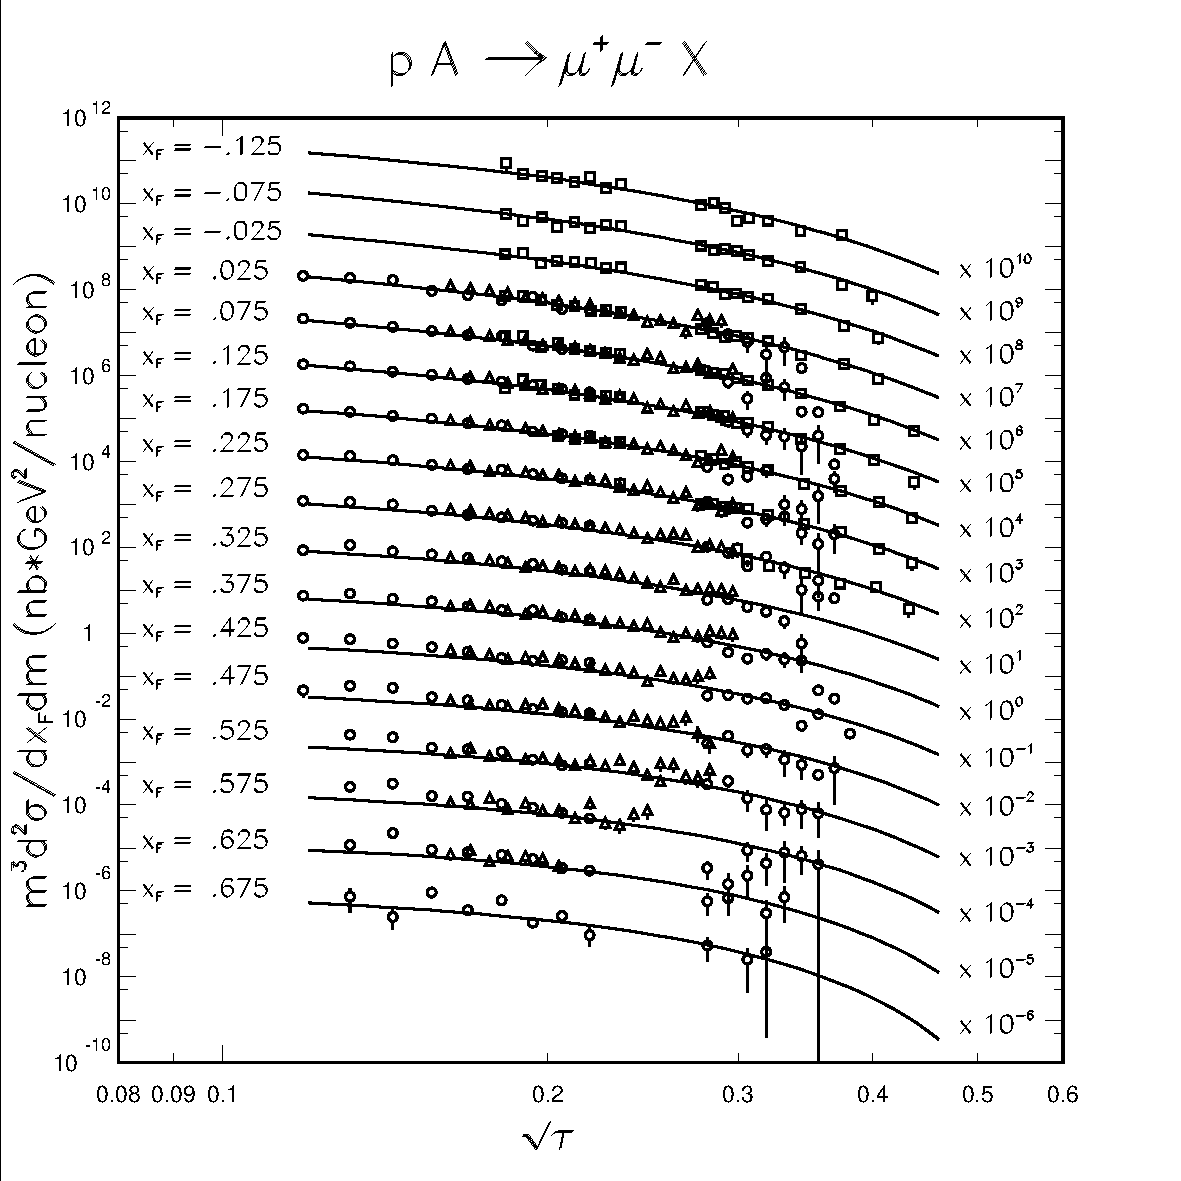
\includegraphics[width=0.5\linewidth]{DY_scaling}
	\caption{Compilation of data on Drell-Yan process, and compared with NLO calculations.
		Taken from Ref.~\cite{mcgaughey1999}}
	\label{fig:DY_scaling}
\end{figure}

One of the advantages of Drell-Yan over DIS is the explicit separation of the quark
and anti-quark distributions in \cref{eq:DY_cs}. At large $x$, DIS cross section
is dominated by the valence quark distribution. On the other hand, in the region $x_1 \gg x_2$,
the valence quark in the Drell-Yan process is more likely to come from the beam
hadron, and the anti-quark is more likely to come from the target hadron. Hence,
Drell-Yan can be more sensitive to the anti-quark distribution than DIS. In
particular, for high $x_F$ and using the fact there are two up valence quarks in
protons, the $(p+d)/2(p+p)$ Drell-Yan cross section ratio at leading order
can be approximated as
\begin{equation}
	\frac{\sigma^{p+d}}{2\sigma^{p+p}} \approx \frac{1}{2} \left( 1+ \frac{\bar{d}\left(x_2\right)}{\bar{u}\left(x_2\right)} \right).
\end{equation}
Thus the Drell-Yan process has been used in many experiments to probe the sea-quarks
asymmetry, with the goal of measuring the $x$ dependence of the sea-quark asymmetry
instead of only the integral as with the Gottfried sum rule.


\section{E866/NuSea}
\label{sec:E866}
Utilizing the sensitivity of the Drell-Yan process to the sea-quark asymmetry,
the E866/NuSea experiment \cite{towell2001} was designed to measure the $(p+d)/2(p+p)$
Drell-Yan cross section ratio over a broad range of $x$. The
experiment utilized the \SI{800}{\GeV} proton beam from the Tevatron on liquid
hydrogen and deuterium targets. The measured deuteriuym over hydrogen cross section
ratio from E866/NuSea is shown in \cref{fig:e866_result}. At low $x$, the ratio is consistent
with a symmetric sea, and the asymmetry becomes larger as $x$ increases, as expected from
the model predictions. However, at $x_2>0.25$ the cross section ratio
drop off below unity, suggesting the $\bar{d}/\bar{u}$
ratio drop off below 1, which could not be explained by models at the time.
Due to the large uncertainty on the data points at large $x_2$, a new
experiment was needed to explore sea quark asymmetry the high $x$ region with better
accuracy.
\begin{figure}[htbp!]
	\centering
	\begin{subfigure}{0.45\linewidth}
		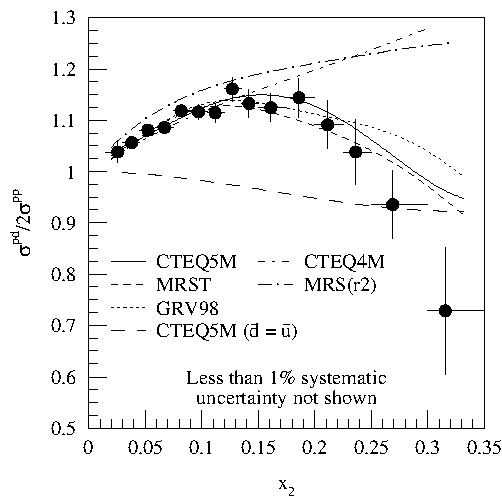
\includegraphics[width=\linewidth]{e866_csr}
		\caption{$(p+p)/2(p+d)$ Drell-Yan cross section ratio}
		\label{subfig:e866_csr}
	\end{subfigure}
	\begin{subfigure}{0.45\linewidth}
		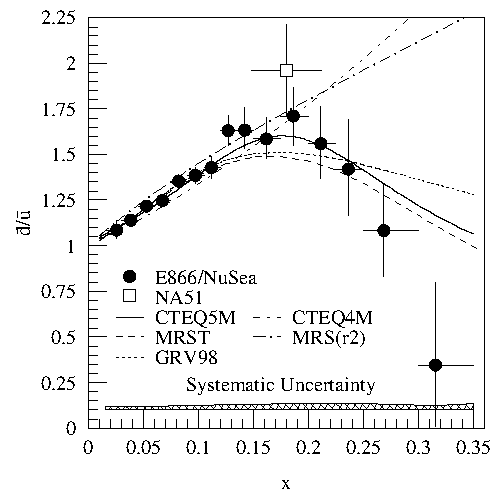
\includegraphics[width=\linewidth]{e866_dbarubar}
		\caption{$\bar{d}/\bar{u}$ extracted from E866 result.}
		\label{subfig:e866_dbarubar}
	\end{subfigure}
	\caption{The E866 result taken from Ref.~\cite{towell2001}}
	\label{fig:e866_result}
\end{figure}

\section{Origin of the \texorpdfstring{$\bar{d}/\bar{u}$}{dbar/ubar} Asymmetry }
After the result from NMC and other DIS experiments indicating the violation of the Gottfried sum rule,
various models have been proposed to explain the $\bar{d}/\bar{u}$ asymmetry. One of the early proposal
is by Field and Feynman \cite{field1977}. They suggested that the Pauli blocking effect
could suppress the production of $u\bar{u}$ pairs relative to  $d\bar{d}$ due to the presence of two
valence $u$ quarks in the proton. It was later shown that the effect by Pauli blocking would be small and
may actually have an opposite effect \cite{steffens1997}. Since the contribution from gluon splitting to the
sea quarks is flavor-blind and the mass of $u$ and $d$ quarks are roughly equal, the asymmetry in the
light sea-quarks must originate from a non-perturbative mechanism. Some of the models will be presented
in this section.

\subsection{Meson Cloud Model}
Some of the early models attribute the asymmetry to the existence of a ``pion cloud'' in the proton.
In the meson cloud model \cite{kumano1998} the proton wave function is written as a sum of meson-baryon states
\begin{equation}
	\ket{p} = \sqrt{Z}\ket{p}_{bare} + \sum_{MB}\int \dd{y} \dd[2]{\vec{k}_\perp} \phi_{BM} \left(y, k^2_\perp\right)\ket{M\left(y, \vec{k}_\perp\right);B\left(1-y, -\vec{k}_\perp\right)}
\end{equation}
where $\phi_{BM}$ is the probability amplitude to find a physical nucleon in a state consisting of a virtual
meson $M$ and virtual baryon $B$ with longitudinal momentum fraction $y$ and $1-y$ and transverse momenta
$\vec{k}_\perp$ and $-\vec{k}_\perp$ respectively. $Z$ is the standard wave function normalization factor
and can be interpreted as the probability of finding a bare proton, which only contains a symmetric sea.

The main hypothesis is that the exchanged photon in the DIS process can interact with the partons in the
virtual meson or the virtual
baryon. Therefore, the PDF can be related to the PDF of either the stuck meson or stuck baryon.
\begin{equation}
	f_{i/N}\left(x\right) = f_{i/N}^{\mathrm{bare}}\left(x\right) +  \int^1_x f_{MB/N}\left(y\right) f_{i/M}\left(\frac{x}{y}\right) \frac{\dd{y}}{y} + \int^1_x f_{BM/N}\left(y\right) f_{i/B}\left(\frac{x}{y}\right) \frac{\dd{y}}{y},
\end{equation}
where $f_{MB/N}$ and $f_{BM/N}$ are the splitting function, related to $\phi_{BM}$, and $f_{MB/N}(y)=f_{BM/N}(1-y)$.
If we restrict to $\pi N$ and $\pi\Delta$ states, and using isospin symmetry,
\begin{align}
	f_{\pi^+n/p}=\frac{2}{3} f_{\pi N}                                       & , ~f_{\pi^0 p/p}=\frac{1}{3} f_{\pi N},                                         \\
	f_{\pi^-\Delta^{++}/p}=\frac{1}{2} f_{\pi \Delta}, ~f_{\pi^0 \Delta^+/p} & =\frac{1}{3} f_{\pi \Delta},  ~f_{\pi^+ \Delta^0/p}=\frac{1}{6} f_{\pi \Delta}.
\end{align}
The light sea-quark distribution in the proton is given by
\begin{align}
	\bar{d}(x) & = \left(\frac{5}{6}f_{\pi N} + \frac{1}{3}f_{\pi \Delta}\right)\otimes q^v_\pi + S(x) \\
	\bar{u}(x) & = \left(\frac{1}{6}f_{\pi N} + \frac{2}{3}f_{\pi \Delta}\right)\otimes q^v_\pi + S(x)
	\label{eq:pion_dbub}
\end{align}
where $f\otimes q\equiv \int^1_x \frac{dy}{y}f(y)q\left(\frac{x}{y}\right)$, and $q^v_\pi$ is the valence
quark distribution in pions and $S(x)$ is the flavor symmetric contributions.
The asymmetry in the proton sea arises because of the dominance of the $\pi^+$ among the $\pi N$ states.
However, the effect is slightly reduced by the $\pi\Delta$ configurations, which favors $\bar{u}$ over $\bar{d}$.
As the $\Delta$ baryon is heavier than the proton, the $\pi\Delta$ configurations should be less important than
the $\pi N$ configurations.
If we took the difference $\bar{d}-\bar{u}$, the flavor symmetric contributions $S(x)$ would cancel out.
\Cref{fig:pion_cloud}
shows the predicted $\bar{d}-\bar{u}$ from the meson cloud model, taken from Ref.~\cite{alberg2022}.
\begin{figure}
	\centering
	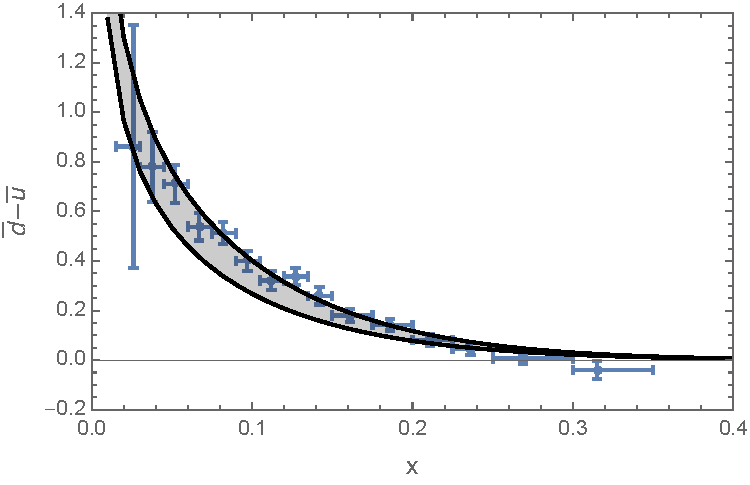
\includegraphics[width=0.5\linewidth]{rediff}
	\caption{The predicted $\bar{d}-\bar{u}$ from the meson cloud model and compared with the E866 results (blue symbol). Taken from Ref.~\cite{alberg2022}}
	\label{fig:pion_cloud}
\end{figure}

\subsection{Chiral Quark Model}
Similar to the meson cloud model, the chiral quark model \cite{li1998} attributes the sea quarks to
the presence of Goldstone bosons in the nucleon. However, the Goldstone bosons in chiral quark model
are emitted from the valence quarks. The quark helicity would also be modified by the emission of a
spin-zero meson in P-wave, as indicated by the subscripts.
\begin{equation}
	q_{\pm} \rightarrow GB + q^\prime_\mp \rightarrow \left(q q^\prime\right)_0 q_{\mp}^\prime.
\end{equation}
For example, after one emission, the $u$ quark wavefuction would have the following components
\begin{equation}
	\Psi\left(u\right) \sim \left[d\pi^+ + s K^+ + u \left(\frac{\pi^0}{\sqrt{2}} + \frac{\eta}{\sqrt{6}}\right)\right],
\end{equation}
which can be expressed in terms of the quark contents by using $\pi^+ = u\bar{d}$ and $K^+ = u\bar{s}$. etc.
The probability of the transitions is given by the squaring the wavefunction, and if
\begin{equation}
	Prob\left[ u_+ \rightarrow \pi^+d_-\right] \equiv a,
\end{equation}
and using isospin asymmetry to determine the $d$ quark wavefucntion, the number of antiquark after one emission
by the initial $(2u+d)$ valence quarks in the proton is given by
\begin{equation}
	\begin{aligned}
		\bar{u} \equiv \int^1_0 \dd{x}\bar{u}(x) & = 2\cross\frac{4}{9}a +a+\frac{1}{9}a = 2a,                         \\
		\bar{d} \equiv \int^1_0 \dd{x}\bar{d}(x) & = 2\cross\left(a+\frac{1}{9}a\right) + \frac{4}{9}a = \frac{8}{3}a.
	\end{aligned}
\end{equation}
Therefore the model predicts a light sea-quark asymmetry $\bar{d}/\bar{u} =\frac{4}{3} $.
Unlike the meson cloud model, the Goldstone boson in the chiral quark model are emitted
by the valance quarks, which only carry a fraction of the total hadron model.
Therefore the boson in the chiral quark model would necessarily carry a smaller momentum than
it would in the meson cloud model, and the sea-quark distributions would peak at a lower value of $x$ \cite{szczurek1996,peng1998}.



\subsection{Statistical Model}
In the statistical model\cite{bourrely2015}, the nucleon is viewed as a gas of massless partons in equilibrium in
a finite volume. And the parton distributions at the initial scale would then be proportional to
\begin{equation}
	\left[ \exp\left[\left(x-X_{0p}\right)/\bar{x}\right] \pm 1 \right]^{-1},
\end{equation}
where the plus sign for the quarks and antiquarks corresponds to a Fermi-Dirac distribution and
the minus sign for gluons corresponds to a Bose-Einstein distribution. The constant $X_{0p}$
plays the role of the thermodynamic potential of the parton $p$ and $\bar{x}$ is the universal
temperature.

In this model, the potential of a quark $q_i^h$ with helicity $h$ has an opposite sign to that of the
potential of the corresponding antiquark $q_i^{-h}$ with helicity $-h$
\begin{equation}
	X_{0q}^h = -X_{0\bar{q}}^{-h}.
	\label{eq:stat_potential}
\end{equation}
Since there are more $u$ quarks than $d$ quarks in the proton, one would expect
\begin{equation}
	X_{0u}^+ + X_{0u}^- > X_{0d}^+ + X_{0d}^-,
\end{equation}
and combining with \cref{eq:stat_potential}, one would expect $\bar{d} > \bar{u}$ in the proton.
And this is shown in \cref{fig:stat_dbub}.
\begin{figure}
	\centering
	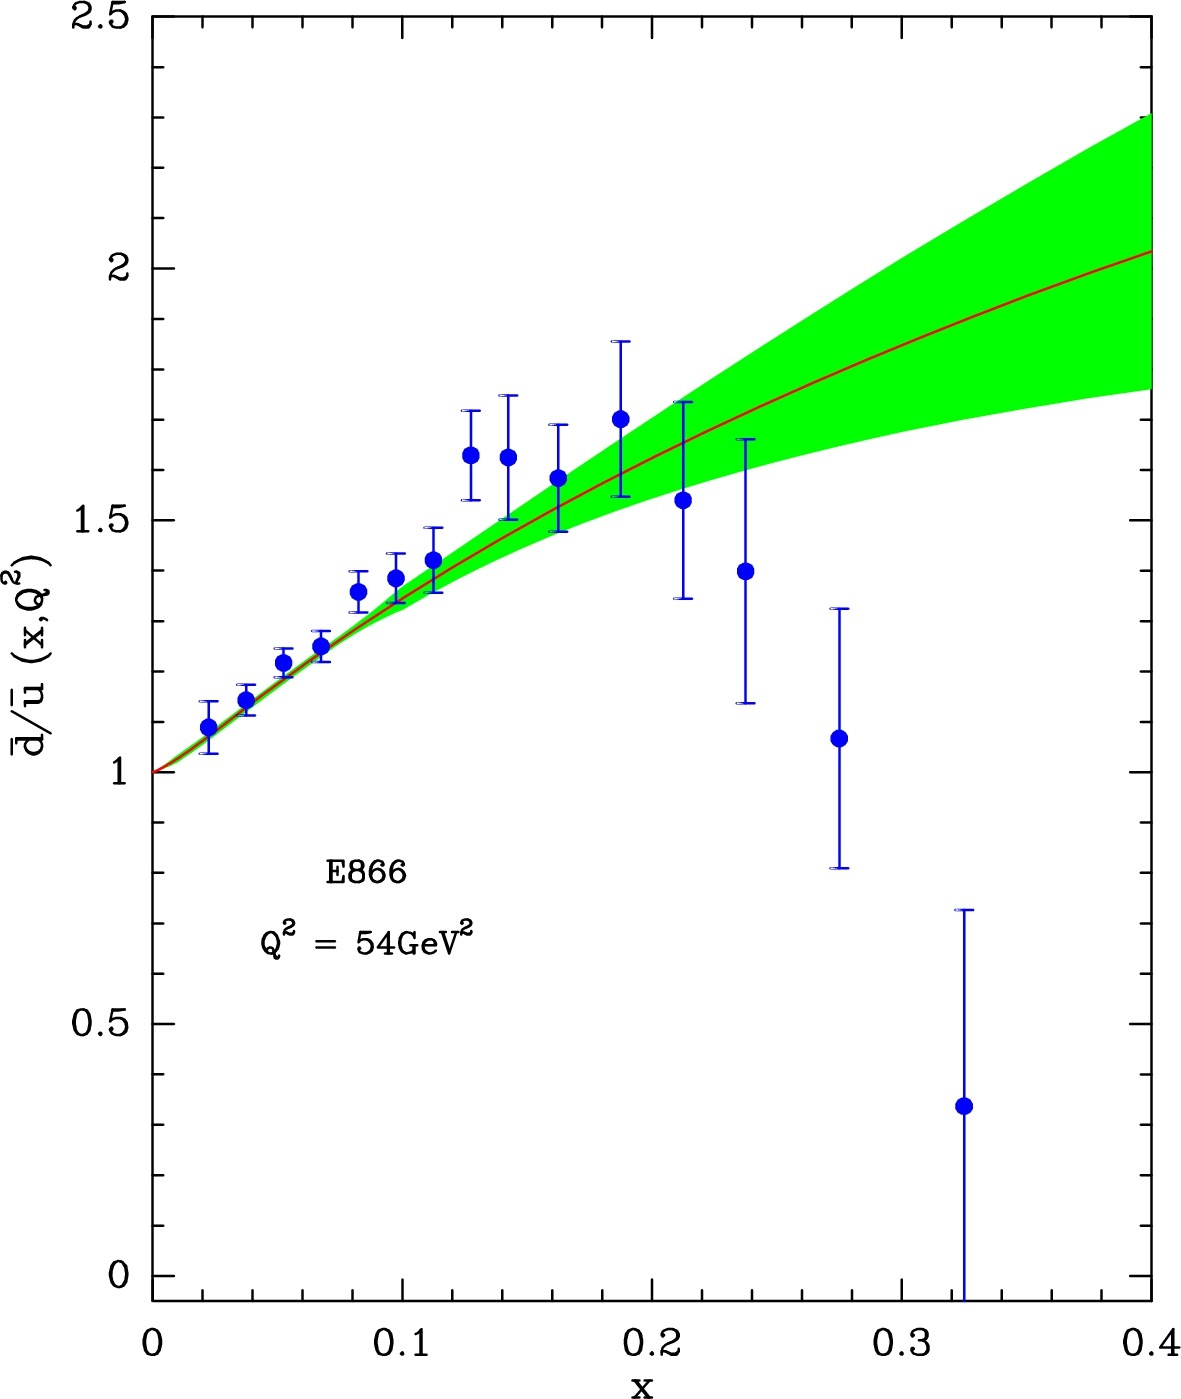
\includegraphics[width=0.5\linewidth]{statistical_model}
	\caption{The extracted light sea-quark asymmetry from the statistical model and compared with E866. Taken
		from Ref.~\cite{soffer2019}.}
	\label{fig:stat_dbub}
\end{figure}


\subsection{Five-quark Intrinsic Sea Model}
In the 1980s, Brodsky, Hoyer, Peterson and Sakai (BHPS) \cite{brodsky1980}, proposed
the possible existence of a significant $\ket{uudc\bar{c}}$ five-quark Fock state component
in the proton in order to explain the larger than expected charmed hadrons production rate.

For a $\ket{uudQ\bar{Q}}$ proton Fock state, the probability for quark $i$ to carry a momentum
fraction $x_i$ is given by
\begin{equation}
	P\left(x_1,\cdots,x_2\right)=N_5 \delta\left(1-\sum^5_{i=1}x_i\right)\left[m_p^2-\sum^5_{i=1}\frac{m_i^2}{x_i}\right]^{-2},
\end{equation}
where the delta function ensures momentum conservation. $N_5$ is the normalization factor,
and $m_i$ is the mass of quark $i$.

\pdfmargincomment{this model can at most predict the x dependence of dbar -ubar, but not the magnitude. It is worth keeping?}

Since the BHPS model also predicts the probability for the $\ket{uudQ\bar{Q}}$ configuration to
be inversely proportional to the mass of the quark $Q$, the intrinsic sea can have important
contribution to the light sea-quarks. In Ref.~\cite{chang2011,chang2011a}, the BHPS model
was extend to the light quark sector and is compared with experimental measurements.
Recent global analysis from NNPDF \cite{ball2022} and measurement from the LHCb \cite{aaij2022}
has shown the importance of intrinsic charm in the proton.



\subsection{Lattice QCD}
Lattice QCD calculations of the $\bar{d} - \bar{u}$ based on the Large Momentum Effective
theory (LaMET) \cite{ji2021,constantinou2021} have become available recently by two different groups,
LP3\cite{chen2018} and ETMC\cite{alexandrou2018}.
The parton distribution functions described quarks and gluons in hadrons traveling at infinite
momentum. The principle for LaMET comes from the observation that the structure of the proton is
approximately independent of its momentum so long as it is much larger than the strong interaction
scale or its mass. Therefore the partonic structure can be calculated for a proton with
moderately-large momentum and taking the limit of the proton momentum to infinity.

\begin{figure}[h!]
	\centering
	\begin{subfigure}{0.45\linewidth}
		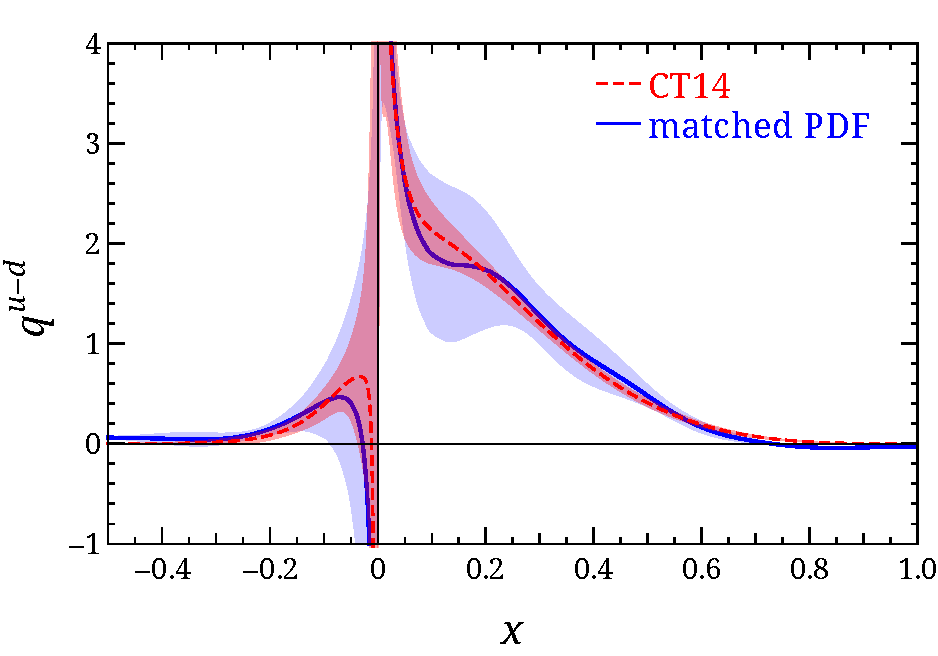
\includegraphics[width=0.9\linewidth]{LP3-PDF-CT14}
	\end{subfigure}
	\begin{subfigure}{0.45\linewidth}
		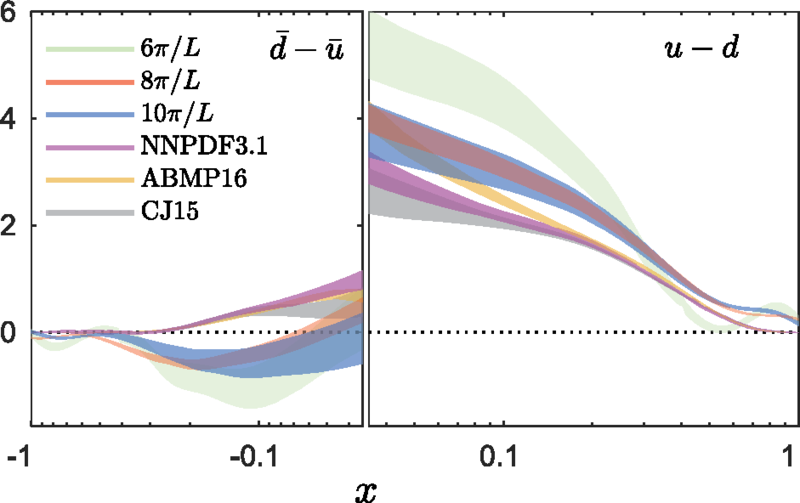
\includegraphics[width=0.9\linewidth]{alexandrou2018}
	\end{subfigure}
	\caption{The calculated isovector PDF from the LP3 collaboration (left)
		\cite{chen2018} and ETMC (right)\cite{alexandrou2018}.
		The negative $x$ region denote $\bar{d}-\bar{u}$ at $\left|x\right|$.}
	\label{fig:lamet}
\end{figure}
LaMET are typically used to calculate flavor non-singlet quantities such as $u-d$ and $\bar{d}-\bar{u}$,
as the disconnected diagram would cancel out in the calculation.
\Cref{fig:lamet} shows the result using LaMET from two different groups and are compared with
different global PDF extractions. While the result by the LP3 collaboration
is in good agreement with CT14, the result from the ETMC group differs from the PDFs,
especially in the antiquark region.




\chapter{Charmonium Production}
\label{ch:jpsi}
Another process for probing the nucleon structure is via the charmonium production \cite{peng1995,chang2020}.
Unlike DIS and Drell-Yan, the charmonium production involves the strong interaction
at leading-order. Therefore it can be used to probe the gluon structure, which is
less sensitive in DIS or Drell-Yan, and the quark anti-quark structure. However,
because of the non-perturbative nature of QCD, there are various models for
calculating the charmonium production. The models usually separate the production
mechanism into two parts, the production of heavy-quark pairs and their subsequent
hadronization into quarkonium states. One of the early approaches is the Color
Evaporation method (CEM) \cite{einhorn1975,bodwin1995}. The heavy-quark
pairs production is expanded in terms of the strong coupling constant $\alpha_s$
and is calculated with perturbative QCD (pQCD). CEM then assumes a constant
probability $F$ for the $c\bar{c}$ pairs to hadronize into a specific charmonium
state and this probability is independent of the kinematics or the production
subprocess. The charmonium production cross section in the CEM framework can be
expressed as
\begin{equation}
	\begin{split}
		\left.\frac{d\sigma}{dx_F}\right|_{J/\Psi} &= F \sum_{i,j = q,\bar{q},G}\int^{2m_D}_{2m_c} dM_{c\bar{c}}  \frac{2M_{c\bar{c}}}{s\sqrt{x_F^2+4M_{c\bar{c}}^2/s}}\\
		&\cross f_{i/A}\left(x_1,\mu_F\right)f_{j/B}\left(x_2,\mu_F\right)\sigma\left[ij\rightarrow c\bar{c}X\right]\left(x_1P_A,x_2P_B,\mu_F,\mu_R \right),
	\end{split}
\end{equation}
where $i$,$j$ denote the type of interacting partons. At leading-order, the
$c\bar{c}$ pairs are produced via two subprocesses, gluon fusion and
quark-antiquark annihilation, as illustrated in \cref{fig:charmonium}.
\begin{figure}[htpb!]
	\centering
	\begin{subfigure}{0.4\linewidth}
		\begin{subfigure}{\linewidth}
			\begin{tikzpicture}
 \tikzstyle{every node}=[font=\large]
    \begin{feynman}
    \vertex  (a1);
    \vertex [right= of a1, blob] (a2) {};
    \vertex [right= 4cm of a2] (a3) ;
    \vertex [below= 2cm of a1] (b1);
    \vertex [below= 2cm of a2,blob] (b2) {};
    \vertex[below= 2cm of a3] (b3);
    \vertex  at ($(b2) + (1.5cm , +1cm)$) [dot] (d);
    \vertex [right= 1cm of d] (d1);
     \vertex at ($(d1) + (1.5cm , +0.7cm)$) (c1) {$c$};
     \vertex at ($(d1) + (1.5cm , -0.7cm)$) (c2) {$\bar{c}$};
     \diagram*{
     (a1) --[fermion](a2),
     (a2) --[double](a3),
     (b1) --[fermion](b2),
     (b2) --[double](b3),
     (b2) --[gluon, edge label'=\(g\)] (d),
     (a2) --[gluon, edge label=\(g\)](d),
     (d) --[gluon](d1),
     (c2) --[fermion] (d1);
     (d1) --[fermion] (c1);
     };
    \end{feynman}
\end{tikzpicture}
		\end{subfigure}
		\begin{subfigure}{\linewidth}
			\begin{tikzpicture}
\tikzstyle{every node}=[font=\large]
    \begin{feynman}
    \vertex  (a1);
    \vertex [right= of a1, blob] (a2) {};
    \vertex [right= 4cm of a2] (a3) ;
    \vertex [below= 2cm of a1] (b1);
    \vertex [below= 2cm of a2,blob] (b2) {};
    \vertex [below= 2cm of a3] (b3);
    \vertex  at ($(b2) + (1.5cm , +0.666cm)$) [dot] (d);
    \vertex [above= 0.668cm of d] (d1);
     \vertex [right= 2.25cm of d1] (c1) {$c$};
     \vertex [right= 2.25cm of d] (c2) {$\bar{c}$};
     \diagram*{
     (a1) --[fermion](a2),
     (a2) --[double](a3),
     (b1) --[fermion](b2),
     (b2) --[double](b3),
     (b2) --[gluon, edge label=$g$] (d),
     
     (a2) --[gluon, edge label'=$g$](d1),
     (d) --[fermion](d1),
     (d1) --[fermion] (c1);
     (c2) --[fermion] (d);
     };
    \end{feynman}
\end{tikzpicture}
		\end{subfigure}
		\caption{gluon fusion\label{subfig:gluon}}
	\end{subfigure}
	\quad
	\begin{subfigure}{0.4\linewidth}
		\begin{tikzpicture}
\tikzstyle{every node}=[font=\large]
    \begin{feynman}
    \vertex  (a1);
    \vertex [right= of a1, blob] (a2) {};
    \vertex [right= 4cm of a2] (a3) ;
    \vertex [below= 2cm of a1] (b1);
    \vertex [below= 2cm of a2,blob] (b2) {};
    \vertex[below= 2cm of a3] (b3);
    \vertex  at ($(b2) + (1.5cm , +1cm)$) [dot] (d);
    \vertex [right= 1 cm of d] (d1);
     \vertex at ($(d1) + (1.5cm , +0.7cm)$) (c1) {$c$};
     \vertex at ($(d1) + (1.5cm , -0.7cm)$) (c2) {$\bar{c}$};
     \diagram*{
     (a1) --[fermion](a2),
     (a2) --[double](a3),
     (b1) --[fermion](b2),
     (b2) --[double](b3),
     (d) --[fermion, edge label=$\bar{q}$] (b2),
     (a2) --[fermion, edge label=$q$](d),
     (d) --[gluon](d1),
     (c2) --[fermion] (d1);
     (d1) --[fermion] (c1);
     };
    \end{feynman}
\end{tikzpicture}
		\caption{quark-antiquark annihilation\label{subfig:qqbar}}
	\end{subfigure}
	\caption{The Feynman diagram for $c\bar{c}$ pair production}
	\label{fig:charmonium}
\end{figure}
The calculated cross section for $J/\Psi$ production in $p+p$ at 120 GeV using
CEM is shown in \cref{fig:cem_cs}. The relative importance of gluon fusion
and quark-antiquark annihilation is a strong function of $x_F=2P_L/\sqrt{s}$,
where $P_L$ is the longitudinal momentum of the $J/\Psi$ meson in the
hadron-hadron center-of-mass frame and $\sqrt{s}$ is the total energy in this
frame. At large $x_F$, the quark-antiquark annihilation is the dominant subprocess.
\begin{figure}[h!]
	\centering
	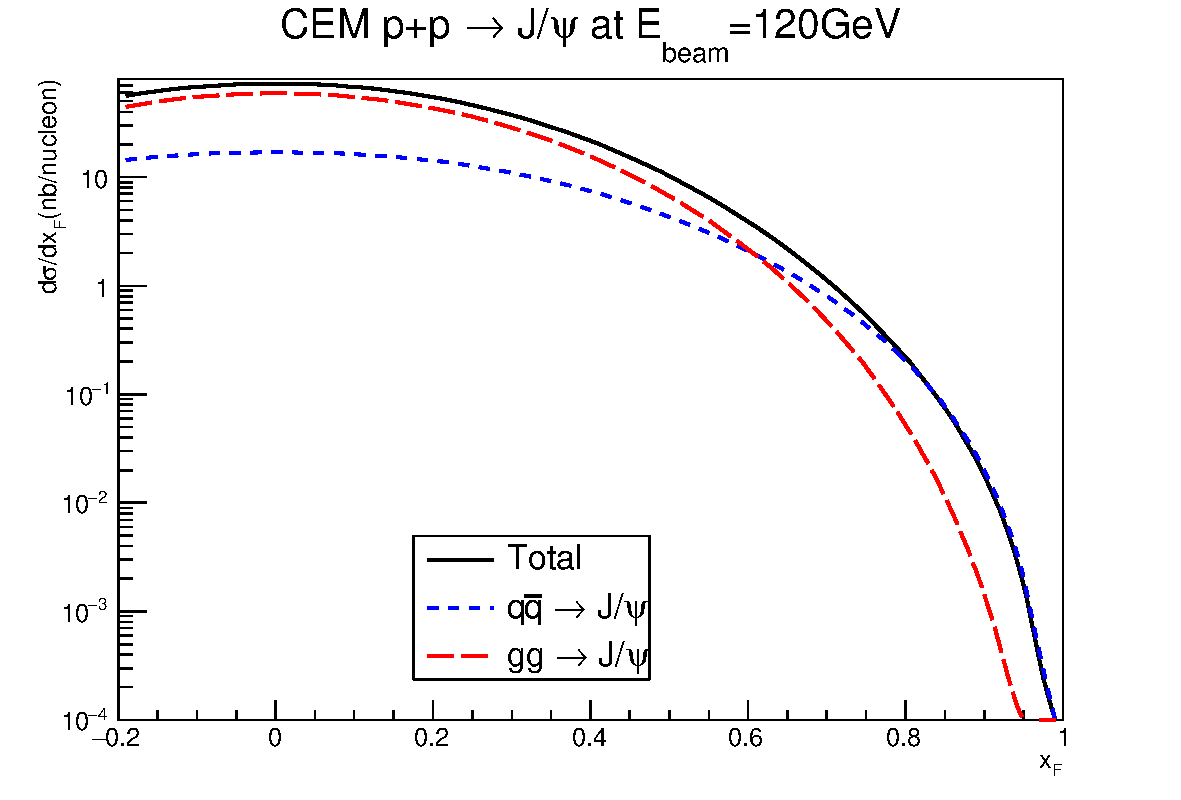
\includegraphics[width=0.45\linewidth]{pp_norm_cs_NLO_pp}
	\caption{Calculated cross section for $J/\Psi$ production using CEM model with CT14NLO PDF.
		The CEM code is obtained from Ref.~\cite{mangano1993}.}
	\label{fig:cem_cs}
\end{figure}

Another theoretical model for quarkonium productions is the non-relativistic
QCD (NRQCD) \cite{bodwin1995}. Unlike CEM, the probability of
hadronization depends on the color and spin state of the $c\bar{c}$ pairs and
is described by various long-distance matrix elements (LDMEs). The quarkonium
production cross section in this framework is given as
\begin{equation}
	\begin{split}
		\frac{d\sigma^H}{dx_F} &=\sum_{i,j = q,\bar{q},G}\int^1_0 dx_1 dx_2 \delta(x_F-x_1+x_2)\\
		&\cross f_{i/A}\left(x_1,\mu_F\right)f_{j/B}\left(x_2,\mu_F\right)\hat{\sigma}\left[ij\rightarrow H\right]\left(x_1P_A,x_2P_B,\mu_F,\mu_R , m_c\right),
	\end{split}
\end{equation}
\begin{equation}
	\hat{\sigma}\left[ij\rightarrow H\right]= \sum_n C^{ij}_{c\bar{c}\left[n\right]}\left(x_1P_A,x_2P_B,\mu_F,\mu_R , m_c\right)\expval{O^H_n \left[^{2S+1}L_J\right]},
\end{equation}
where the $c\bar{c}$ pair is labeled by its color ($n$), spin ($S$), orbital
angular momentum ($L$) and total angular momentum ($J$). The coefficient
$C^{ij}_{c\bar{c}\left[n\right]}$ describes the production of $c\bar{c}$ pair
with specific color-spin state and is calculated perturbatively in powers of
$\alpha_s$ using pQCD. The LDME $\expval{O^H_n \left[^{2S+1}L_J\right]}$ accounts
for the hardronization probability for a specfic $c\bar{c}$ state into the
charmonium state $H$. These LDMEs are obtained by fitting to data and assumed to
be universal, independent of beam or target hadrons and the energy scale. The
calculated cross sections for $J/\Psi$ and $\Psi'$ production using NRQCD for
$p+p$ at 120 GeV are shown in \cref{fig:NRQCD_cs}. In this model, quark-antiquark
annihilation is more important than suggested by CEM. This model also suggests
that the relative importance of the two subprocess depends on the charmonium state.
In particular, \cref{fig:NRQCD_cs} shows that the quark-antiquark annihilation
is the dominant process for $\Psi^\prime$ production.
\begin{figure}[h!]
	\centering
	\begin{subfigure}{0.45\linewidth}
		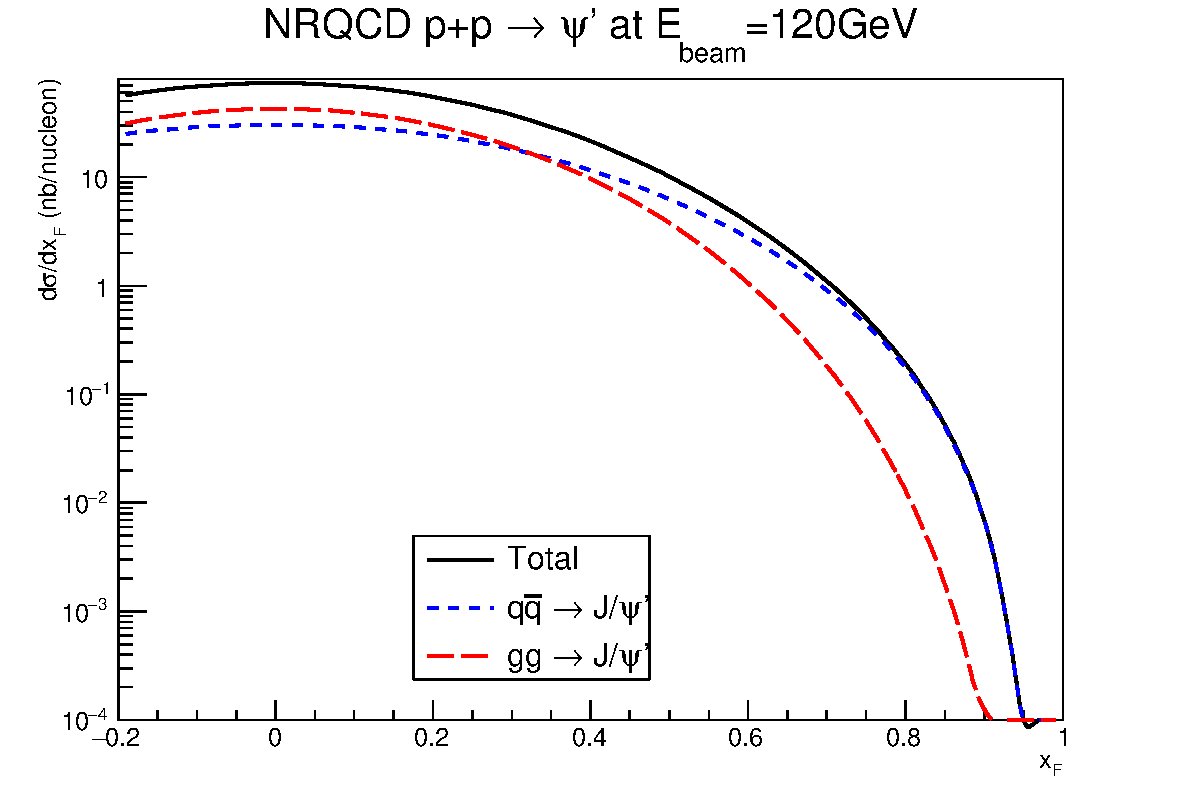
\includegraphics[width=\linewidth]{jpsi_cs_pp}
		\caption{$J/\Psi$ production}
	\end{subfigure}
	\quad
	\begin{subfigure}{0.45\linewidth}
		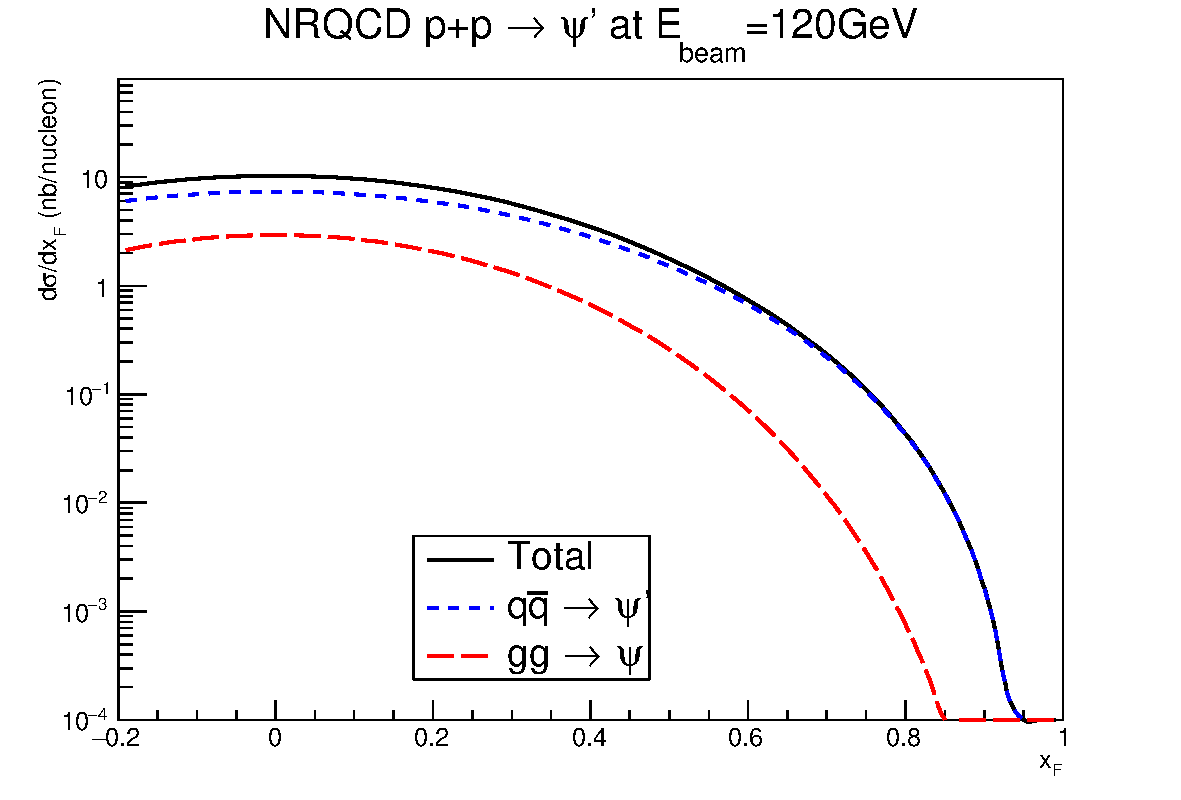
\includegraphics[width=\linewidth]{psip_cs_pp}
		\caption{$\Psi'$ production}
	\end{subfigure}
	\caption{Calculated cross section for charmonium production using NRQCD model
		\cite{chang2021}. CT14nlo is used as the proton PDF. The LDMEs used are
		taken from table \num{4} in Ref.~\cite{hsieh2021}, and are obtained from a
		global fit to fixed-target charmonium production data. }
	\label{fig:NRQCD_cs}
\end{figure}

\pdfmargincomment{what is physical significant of the nuclear dependence}

\ifSubfilesClassLoaded{ \printbibliography[heading=bibintoc,title={References}]}{}

\end{document}
